% ******************************* PhD Thesis Template **************************
% Please have a look at the README.md file for info on how to use the template

\documentclass[a4paper,12pt,times,numbered,print,index]{PhDThesisPSnPDF}

\usepackage{amsmath}
\usepackage{tikz}
\usetikzlibrary{automata,arrows,positioning,calc}

% ******************************************************************************
% ******************************* Class Options ********************************
% *********************** See README for more details **************************
% ******************************************************************************

% `a4paper'(The University of Cambridge PhD thesis guidelines recommends a page
% size a4 - default option) or `a5paper': A5 Paper size is also allowed as per
% the Cambridge University Engineering Deparment guidelines for PhD thesis
%
% `11pt' or `12pt'(default): Font Size 10pt is NOT recommended by the University
% guidelines
%
% `oneside' or `twoside'(default): Printing double side (twoside) or single
% side.
%
% `print': Use `print' for print version with appropriate margins and page
% layout. Leaving the options field blank will activate Online version.
%
% `index': For index at the end of the thesis
%
% `draftclassic': For draft mode without loading any images (same as draft in book)
%
% `draft': Special draft mode with line numbers, images, and water mark with
% timestamp and custom text. Position of the text can also be modified.
%
% `abstract': To generate only the title page and abstract page with
% dissertation title and name, to submit to the Student Registry
%
% `chapter`: This option enables only the specified chapter and it's references
%  Useful for review and corrections.
%
% ************************* Custom Page Margins ********************************
%
% `custommargin`: Use `custommargin' in options to activate custom page margins,
% which can be defined in the preamble.tex. Custom margin will override
% print/online margin setup.
%
% *********************** Choosing the Fonts in Class Options ******************
%
% `times' : Times font with math support. (The Cambridge University guidelines
% recommend using times)
%
% `fourier': Utopia Font with Fourier Math font (Font has to be installed)
%            It's a free font.
%
% `customfont': Use `customfont' option in the document class and load the
% package in the preamble.tex
%
% default or leave empty: `Latin Modern' font will be loaded.
%
% ********************** Choosing the Bibliography style ***********************
%
% `authoryear': For author-year citation eg., Krishna (2013)
%
% `numbered': (Default Option) For numbered and sorted citation e.g., [1,5,2]
%
% `custombib': Define your own bibliography style in the `preamble.tex' file.
%              `\RequirePackage[square, sort, numbers, authoryear]{natbib}'.
%              This can be also used to load biblatex instead of natbib
%              (See Preamble)
%
% **************************** Choosing the Page Style *************************
%
% `default (leave empty)': For Page Numbers in Header (Left Even, Right Odd) and
% Chapter Name in Header (Right Even) and Section Name (Left Odd). Blank Footer.
%
% `PageStyleI': Chapter Name next & Page Number on Even Side (Left Even).
% Section Name & Page Number in Header on Odd Side (Right Odd). Footer is empty.
%
% `PageStyleII': Chapter Name on Even Side (Left Even) in Header. Section Number
% and Section Name in Header on Odd Side (Right Odd). Page numbering in footer

% Uncomment to change page style
%\pagestyle{PageStyleII}

% ********************************** Preamble **********************************
% Preamble: Contains packages and user-defined commands and settings
% ******************************************************************************
% ****************************** Custom Margin *********************************
\ifsetCustomMargin%
  \RequirePackage[left=37mm,right=30mm,top=35mm,bottom=30mm]{geometry}
  \setFancyHdr%
\fi

\raggedbottom%

% *****************************************************************************
% **************************** Custom Packages ********************************

% ********************Captions and Hyperreferencing / URL **********************
\RequirePackage[labelsep=space, tableposition=top]{caption}
\renewcommand{\figurename}{Fig.}

% *************************** Graphics and figures *****************************
\usepackage{subcaption}

% ********************************** Tables ************************************
\usepackage{booktabs} % For professional looking tables
\usepackage{multirow}
\usepackage{caption}
\usepackage{anyfontsize}
\usepackage{bbm}
\usepackage{commath}
\usepackage{amsmath}
\usepackage{mathrsfs}
\usepackage{tikz}
\usepackage{bookmark}
\usetikzlibrary{automata,arrows,positioning,calc,shapes.geometric}

% *********************************** SI Units *********************************
\usepackage{siunitx}

% *****************************************************************************
% *************************** Bibliography  and References ********************
\addbibresource{References/references.bib}
\bibliography{References/references}


% ********************** TOC depth and numbering depth *************************
\setcounter{secnumdepth}{4}
\setcounter{tocdepth}{4}

% *****************************************************************************
% ******************* Better enumeration my MB*************
\usepackage{enumitem}
\usepackage{hyperref}

% ************************ Thesis Information & Meta-data **********************
% Thesis title and author information, refernce file for biblatex
% ************************ Thesis Information & Meta-data **********************
%% The title of the thesis
\title{Hidden Markov Models for Cryptocurrency Trading}

%% The full name of the author
\author{Bc. Adam Pešek}

%% Faculty (eg. Faculty of Technology, Engineering, Maths)
\faculty{Faculty of Finance and Accounting}

%% Department (eg. Department of Engineering, Maths, Physics)
\dept{Department of Banking and Insurance}

%% Field of study (eg. Engineering, Maths, Physics)
\field{Financial Engineering}

%% University and Crest
\university{Prague University of Economics and Business}

% Crest minimum should be 30mm.
\crest{
\includegraphics[width=0.47\textwidth]{VSE_logo_EN_circle_black.pdf}}

%% Supervisor (optional)
\supervisor{Ing. Milan Fičura, PhD.}

%% Full title of the Degree
\degreetitle{Engineer}

%% City of University
\city{Prague}

%% Submission date
% Default is set as {\monthname[\the\month]\space\the\year}
\degreedate{September 2023} 

%% Meta information
\subject{LaTeX} 

\keywords{{LaTeX} {Master Thesis} {Engineering} {Prague University of Economics and Business}}


% ***************************** Abstract Separate ******************************
% To printout only the titlepage and the abstract with the PhD title and the
% author name for submission to the Student Registry, use the `abstract' option in
% the document class.

\ifdefineAbstract
 \pagestyle{empty}
 \includeonly{Declaration/declaration, Abstract/abstract}
\fi

% ***************************** Chapter Mode ***********************************
% The chapter mode allows user to only print particular chapters with references
% Title, Contents, Frontmatter are disabled by default
% Useful option to review a particular chapter or to send it to supervisior.
% To use choose `chapter' option in the document class

\ifdefineChapter
 \includeonly{Chapter3/chapter3}
\fi

% ******************************** Front Matter ********************************
\begin{document}

\frontmatter

\maketitle

% ******************************* Thesis Dedidcation ********************************

\begin{dedication} 

I would like to dedicate this thesis to my loving parents \dots

\end{dedication}


% ******************************* Thesis Declaration ***************************

\begin{declaration}

I hereby declare that the master thesis "Hidden Markov Models for Cryptocurrency Trading" presented herein is my own work, 
or fully and specifically acknowledged wherever adapted from other sources. 
This work has not been published or submitted elsewhere for the requirement of a degree program. 

\end{declaration}


% ************************** Thesis Acknowledgements **************************

\begin{acknowledgements}      

\begin{singlespace}
    \begin{center}
    \definecolor{color_29791}{rgb}{0,0,0}
    \definecolor{color_156895}{rgb}{0.501961,0.501961,0.501961}
    \definecolor{color_275101}{rgb}{1,0,1}
    \definecolor{color_204026}{rgb}{0.709804,0.031373,0.180392}
    \definecolor{color_97849}{rgb}{0.266667,0.329412,0.415686}
    
    \begin{picture}(-5,0)(2.5,0)
    \put(-200,-380){\fontsize{18}{1}\usefont{T1}{cmr}{b}{n}\selectfont\color{color_29791}Čestné  prohlášení}
    \put(-175,-400){\fontsize{12}{1}\usefont{T1}{ptm}{m}{n}\selectfont\color{color_29791}Prohlašuji, že jsem diplomovou práci „Uveďte název práce“ vypracoval }
    \put(-200,-420){\fontsize{12}{1}\usefont{T1}{ptm}{m}{n}\selectfont\color{color_29791}samostatně a veškerou použitou literaturu a další prameny jsem řádně označil a uvedl  }
    \put(-200,-440){\fontsize{12}{1}\usefont{T1}{ptm}{m}{n}\selectfont\color{color_29791}v přiloženém seznamu.}
    \put(-175,-560){\fontsize{12}{1}\usefont{T1}{ptm}{m}{n}\selectfont\color{color_29791}V Praze dne 5. května 2023}
    \put(302.4,-572.9609){\fontsize{12}{1}\usefont{T1}{ptm}{m}{n}\selectfont\color{color_29791}.....................................................................}
    \put(382.05,-593.6589){\fontsize{12}{1}\usefont{T1}{cmr}{m}{it}\selectfont\color{color_29791}(podpis autora)}
    \end{picture}
    \end{center}
    \end{singlespace}

\end{acknowledgements}

% ************************** Thesis Abstract *****************************
% Use `abstract' as an option in the document class to print only the titlepage and the abstract.
\begin{abstract}

Hidden Markov model (HMM) is a statistical signal prediction model, which has been widely used to predict economic regimes and stock prices. In this paper, we introduce the application of HMM in trading stocks (with S\&P 500 index being an example) based on the stock price predictions. The procedure starts by using four criteria, including the Akaike information, the Bayesian information, the Hannan Quinn information, and the Bozdogan Consistent Akaike Information, in order to determine an optimal number of states for the HMM. The selected four-state HMM is then used to predict monthly closing prices of the S\&P 500 index. For this work, the out-of-sample R OS 2 , and some other error estimators are used to test the HMM predictions against the historical average model. Finally, both the HMM and the historical average model are used to trade the S\&P 500. The obtained results clearly prove that the HMM outperforms this traditional method in predicting and trading stocks.




\end{abstract}


% *********************** Adding TOC and List of Figures ***********************

\tableofcontents

\listoffigures

\listoftables

% \printnomenclature[space] space can be set as 2em between symbol and description
%\printnomenclature[3em]

\printnomenclature

% ******************************** Main Matter *********************************
\mainmatter

%!TEX root = ../thesis.tex
%*******************************************************************************
%*********************************** First Chapter *****************************
%*******************************************************************************


\chapter{Markov Processes}  %Title of the First Chapter

\ifpdf
    \graphicspath{{Chapter1/Figs/Raster/}{Chapter1/Figs/PDF/}{Chapter1/Figs/}}
\else
    \graphicspath{{Chapter1/Figs/Vector/}{Chapter1/Figs/}}
\fi

\tikzstyle{state}=[shape=circle,draw=blue!50,fill=blue!20]
\tikzstyle{observation}=[shape=rectangle,draw=orange!50,fill=orange!20]
\tikzstyle{lightedge}=[<-,dotted]
\tikzstyle{mainstate}=[state,thick]
\tikzstyle{mainedge}=[<-,thick]


Put here the overall definition for sigma algebra and notation and introduction plus motivation



%********************************** %First Section  **************************************
\section{Discrete-time Markov Chains} %Section - 1.2

Let $\Omega \neq \emptyset$ and $A \subseteq 2^{\Omega}$ be a $\sigma$-algebra on $\Omega$, and $P$ a measure on A with $P(\Omega) = 1$, i.e. $P$ is a {\it probability measure}. Then the triplet $(\Omega, A, P)$ is called a {\it probability space}. Where $\Omega$ denotes a sure event, and it holds that $\forall \omega \in \Omega$ is called an elementary event. Furthermore, $\forall A \in A$ is a random event  so that $P(A)$ is a probability of such a random event. 

Let $I$ be a countable set and $\Theta$ a $\sigma$-algebra on $I$. Each $i \in I$ is called a {\it state} and $(I,\Theta)$ a {\it state-space}. We say that $\lambda = (\lambda_i : i \in I) $ is a measure on I if $0 \leq \lambda_i \leq \infty$. If in addition the {\it total mass} $\sum_{i \in I} \lambda_i = 1$ then $\lambda$ is a {\it distribution} (or probability measure). 

Suppose now that we have two measurable spaces $(\Omega,A)$ and $(I,\Theta)$ and a random variable $X: \Omega \rightarrow I$ assuming that X is measurable. Thus, we call $(I,\Theta)$ a state space and $(\Omega, A)$ an underlying space. Therefore, we may set:

\begin{equation}
\lambda_X(i) = P(X=i)=P(\{\omega: X(\omega)=i\})
\end{equation}

Since we are allowing only for the discrete realizations of the random variable X, given previous assumptions, $\lambda_X(i)$ is a {\it probability mass function}.

Then measure $\lambda$ defines a distribution of $X$. Given such a setting random variable $X$ is assumed to denote random state $i$ with probability $\lambda_i$. 

Let us now assume that we have a sequence of random variables $\{X_t : t \in T\}$ where $T$ is a countable set of time steps.
 We say that $\{X_t : t \in T\}$ is a {\it stochastic process} and if it also holds that $T = \mathbb{N}_0$ then {\it discrete-time stochastic process}.
 In the context of Markov Chains we call measurable space $I$ as a {\it state space} and $X_t$ as a {\it state} at time $t$ respectively.
 Given the initial setup, we may define a {\it discrete-time Markov Chain} as a stochastic process $\{X_t : t \in T\}$ with a state space $I$ and a distribution $\lambda$ such that for all $t \in T$ and $i_0,i_1,\ldots,i_{t+1} \in I$ it holds that:

\begin{equation} \label{DTMC}
P(X_{t+1}=i_{t+1}|X_t=i_t,\ldots,X_0=i_0) = P(X_{t+1}=i_{t+1}|X_t=i_t)
\end{equation}

which holds for all $t \in T$ and $i_0,i_1,\ldots,i_{t+1} \in I$. In other words, the probability of observing a state $i_{t+1}$ at time $t+1$ given the sequence of states $i_0,i_1,\ldots,i_{t+1}$ is equal to the probability of observing a state $i_{t+1}$ at time $t+1$ given only the last observed state $i_t$.
This fundamental relationship is called {\it Markov property}, and it is a consequence of the {\it memoryless property} of Markov Chains. 
Conditional property of Markov Chains may be equivalently expressed using current state as $i \in I$ and a previous state $j \in I$ as:

\begin{equation}
P(X_{t+1}=i|X_t=j) = p_{j,i}(t,t+1)
\end{equation}

where $p_{j,i}(t,t+1)$ is a {\it transition probability} from state $j$ to state $i$ at time $t$ and $t+1$ respectively. Sometimes we refer to these transitions as {\it one-step transitions} since they are only dependent on the previous state.
As an extension of the Markov property we may also define a {\it k-step transition} as a probability of observing a state $i$ at time $t+k$ given the state $j$ at time $t$ as:

\begin{equation}
P(X_{t+k}=i|X_t=j) = p_{j,i}(t,t+k)
\end{equation}

One important distinction is that if the transition probabilities $p_{j,i}(t,t+k)$ do not depend on time $t$ then the Markov Chain is called {\it homogeneous} otherwise these probabilities vary over time, therefore {\it heterogeneous} Markov Chain.
Considering only first order homogeneous Markov Chain we may define a {\it transition matrix} 
$A = (p_{i,j} : i,j \in I)$ as a matrix of transition probabilities between each state $i,j \in I$ such that:

\begin{equation} \label{eq:1.5}
p_{j,i} \geq 0 \quad i,j \in I; \quad \sum_{j \in I} ^{}p_{i,j} = 1, \quad \forall i \in I
\end{equation}

Rectangular matrix $P$ that satisfies property given by Equation \ref{eq:1.5} is called {\it stochastic matrix}. 
Furthermore, we ought to define a probability distribution $\textbf{p} =\{p_i, i \in I\} $ as a vector of probabilities of observing a each state at time $t=0$ such that:

\begin{equation}
p_i = P(X_0=i), \quad i \in I
\end{equation}

and 

\begin{equation}
p_i \geq 0 \quad i \in I; \quad \sum_{i \in I} ^{}p_i = 1
\end{equation}

which is also called {\it initial distribution} of Markov Chain. 

Once we have transition matrix $A$ and initial distribution $\textbf{p}$ that satisfy constraints given by Equation (1.5) and (1.7) respectively,
then $\{X_t,t \in \mathbb{N}_0\}$ is a discrete-time homogeneous Markov Chain with transition matrix $A$ and initial distribution $\textbf{p}$ 
if and only if all finite dimensional distributions of $\{X_t,t \in \mathbb{N}_0\}$ are consistent with the following equation:

\begin{equation}
P(X_{0}=i_0,X_{1}=i_1,\ldots,X_{k}=i_k) = p_{i_0} p_{i_0,i_1} \ldots p_{i_{k-1},i_k}
\end{equation}

where $i_0,i_1,\ldots,i_k \in I$ and $k \in \mathbb{N}_0$. If we abstract from the initial distribution $p$, such equation is also called {\it Chapman-Kolmogorov equation}.
Above stated equation also holds for non-homogeneous Markov Chains with the only difference that the transition probabilities $p_{i,j}$ are time dependent:

\begin{equation}
P(X_{0}=i_0,X_{1}=i_1,\ldots,X_{k}=i_k) = p_{i_0}(0) p_{i_0,i_1}(0,1) \ldots p_{i_{k-1},i_k}(k-1,k)
\end{equation}

another substantial property of homogeneous Markov Chains is that their nth order transition probabilities can be expressed as a product of first order transition probabilities:

\begin{equation}
P(X_{m+n} = j|X_{m} = i) = p_{i,j}^{(n)}, \quad i,j \in I
\end{equation}

where generally $p_{i,j}^{(m+n)} = \sum_{k \in I} p_{i,k}^{(m)} p_{k,j}^{(n)}$ is referred to as {\it Chapman-Kolmogorov equality} and holds for $m,n \in \mathbb{N}_0$ and $P(X_m=i) \geq 0$.


To simply illustrate the idea behind discrete-time homogeneous Markov Chains let us assume a situation where the future market movements transition between a countable number of states $I =$ \{upward, side, downward\} 
and there is a transition matrix A and initial distribution $p$:
\begin{equation}
A =
\begin{pmatrix}
0.1 & 0.4 & 0.5 \\
0.25 & 0.3 & 0.45 \\
0.33 & 0.33 & 0.33 
\end{pmatrix} 
, \quad p = 
\begin{pmatrix}
    0.2 & 0.3 & 0.5 \\
\end{pmatrix}
\end{equation}



Each row represents full set of transition probabilities between states, also visible from $\sum_{j \in I} ^{}p_{i,j} = 1 $, i.e. each row of matrix $A$ represents a conditional probability distribution given $i \in I$. 
Such a relationship can be represented as a diagram indexing each state by U, S and D respectively as follows:

\begin{center}
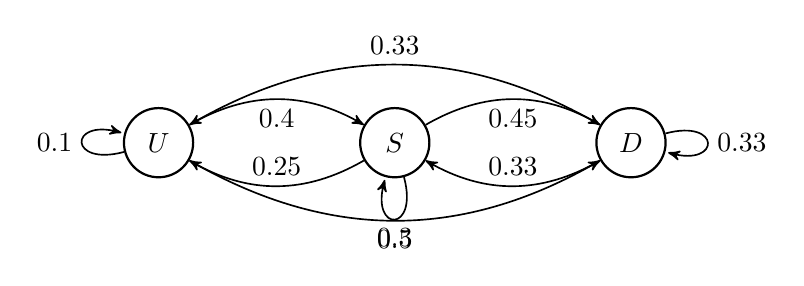
\begin{tikzpicture}[->, >=stealth', auto, semithick, node distance=3cm]
\tikzstyle{every state}=[fill=white,draw=black,thick,text=black,scale=1]
\node[state]    (U)                     {$U$};
\node[state]    (S)[right of=U]   {$S$};
\node[state]    (D)[right of=S]   {$D$};

\path
(U) edge[loop left]     node{$0.1$}         (U)
    edge[bend left,below]     node{$0.4$}     (S)
    edge[bend right,below]      node{$0.5$}      (D)
(S) edge[bend left,below]     node{$0.45$}           (D)
    edge[loop below]     node{$0.3$}           (S)
    edge[bend left, above]     node{$0.25$}           (U)
(D) edge[bend right,above] node{$0.33$}           (U)
    edge[loop right]     node{$0.33$}         (D)
    edge[bend left, above]      node{$0.33$}         (S);
\end{tikzpicture}
\end{center}


 
This may be easily interpreted for each given state. For example if we assume that the market moved upwards on the last trading day there is a 0.1 chance that the market will move in positive direction today, in other words the conditional probability of observing the state U today given the state U yesterday is 0.1. 
On the hand if we suppose that today the market actually transitioned to the state S with probability 0.4 there is now a probability of 0.45 to transition to state D since the future transition is only conditioned by its previous state. 

Up until now we have assumed random variable X that modelled the probability of observing a state $i \in I$ given the initial distribution $\lambda$. We ought to consider  thus we have to allow for a system of discrete random variables that are also identically distributed for each time step $\{X_{t},t \in T \}$, for $\{t_0,t_1,\ldots,t_n\} \subset T$ where $n \in \mathbb{N}_0$.

Suppose now that we have observed a given sequence of states for the last week as $\{U,S,D,D,U\}$, and we would like to know the sequence joint probability given the transition matrix A and initial distribution $p$:

\begin{align*}
P(X_{t_0} = x_0,\ldots,X_{t_n} = x_n|A,p) &= P(X_0 = x_0) \prod_{k=1}^4 P(X_k=x_k|X_{k-1}=x_{k-1})\\
&= p_{x_0} p_{1,2}  p_{2,3}  p_{3,3} p_{3,1} \\
&= 0.2 * 0.4 * 0.45 * 0.33 * 0.33 \\
&= 0.002376
\end{align*}

Where the probability of observing state A is determined by our distribution $\lambda$ evaluated at respective state A since we have no prior knowledge about what exactly happened before $t_0$. 

On the other hand, we might consider a situation in which we have observed such a sequence of events and we need to determine the next state given the sequence. As in the last example, we have our transition matrix P, distribution $\lambda$ and a sequence of events observed until now $\{A,B,C,C,A\}$ for $t_{k-4},\ldots,t_{k}$. Let us also assume that $t_{k+1}$ is a time of next event for which we are trying to determine its probability.

\begin{align}
P(X_{t_{k+1}}|X_{t_{k}},\ldots,X_{t_{k-4}}) &= P(X_{t_{k+1}}|X_{t_{k}})
\end{align}

We know that last observed state was $U$ which directs us straight to the first row of our transition matrix A since from the properties of Markov Processes we know that the next state will depend solely on the present state, 
so we can abstract from the given sequence of past states and focus only on $X_{t_{k}}$. Finally, we may conclude that the most likely future state at time $t_{k+1}$ is D with the probability of 0.5. Formally we may write:

\begin{equation}
 i_{k+1} = \underset{i \in I}{\arg\max} P(X_{t_{k+1}}=i_{k+1}|X_{t_{k}}=i_{k}) \\
\end{equation}

\subsection{Classification of states}

Markov Chains may be classified into several categories based on their properties. 
Firstly, we may distinguish between {\it transient} and {\it recurrent} states and as a convenient notation we will introduce so called {\it return time} $\tau_j$ 
as a random variable that denotes the time of kth return to state $j \in I$:

\begin{equation}
\tau_j(k+1) = \inf \{n \geq \tau_j(k) : X_n =j\}, \quad k \in \mathbb{N}_0
\end{equation}

if $\tau_j(k) \leq \infty$ and we assume that $\inf\{\emptyset\} = \infty$ and $\tau_j(0) = 0$.

This random variable also satisfies properties of {\it recurrence time}. 
Any random variable $\tau:\Omega \to \mathbb{N}_0 \cup \{ \infty \}$ for which outcomes $[\tau = n]$ belong to 
$\sigma$-algebra $\mathcal{F}_n = \sigma(X_0,\ldots,X_n)$ generated by random variables $X_0,X_1, \ldots , X_n$ is called a {\it recurrence time}.

A state $j \in I$ is called {\it transient} if there is a non-zero probability that the process will never return to state $j$ once it has left it, i.e.:

\begin{equation}
P(\tau_j(1) = \infty|X_0=j) > 0, \quad \sum_{n=0}^{\infty} p_{j,j}^{(n)} \leq \infty
\end{equation}

for some $k \in \mathbb{N}_0$. On the other hand, a state $j \in I$ is called {\it recurrent} if it is not transient, i.e.:

\begin{equation}
P(\tau_j(1) \leq \infty|X_0=j) = 1, \quad \sum_{n=0}^{\infty} p_{j,j}^{(n)} = \infty
\end{equation}

We can further distinguish between {\it positive recurrent} if the expected return time is finite $E[\tau_j(1)|X_0=j] < \infty$ and {\it null recurrent} if the expected return time is infinite $E[\tau_j(1)|X_0=j] = \infty$.

Let us make one more distinction regarding a Markov chain states. State is said to be periodic if it can only be revisited (i.e., return to the same state) in multiples of some integer larger than 1. 
The greatest common divisor of these numbers is the period. If the period is larger than 1, the state is called periodic and 
on the contrary, if there is no such integer and the state can be revisited at any time, then the state is called aperiodic. 
If all states in a Markov chain are aperiodic, the Markov chain itself is said to be aperiodic as well. Aperiodicity is a desirable property for a Markov chain because it ensures that the chain does not get trapped in oscillating sequences of states. 
To clarify, aperiodicity does not mean that each state must be reachable from every other state in just one step. It's a more subtle concept, meaning that the greatest common divisor of the lengths of all cycles in the chain must be 1, so that any state can be reached from any other state in a variable number of steps.
Previous properties of states lead us to define ergodic state for which it holds that it needs to be positive recurrent and aperiodic. Such trait is desirable since it implies that the state will be visited infinitely often and the expected time between visits is finite.
That also implies that if all states of a Markov chain are ergodic, then the chain itself is ergodic and irreducible, i.e. all states communicate with each other.

\subsection{Stationary distribution}

A pivotal concept linked to Markov Chains is that of the stationary distribution, a distinct probability 
distribution that remains invariant under the transition dynamics of the chain. 
If we denote $\pi = \{\pi_j,j \in I\}$ as a probability distribution, and it satisfies following equality:

\begin{equation}
    \pi_j = \sum_{i \in I} \pi_i p_{i,j}, \quad j \in I
\end{equation}

then $\pi$ is called a stationary distribution of Markov Chain. That also implies that if the initial distribution of homogeneous Markov Chain is stationary in the sense of Eq. (1.14)
then Markov Chain is called strictly stationary stochastic process since the joint distribution of any finite number of random variables is invariant under the transition dynamics of the chain.
More specifically, for any $n,k \in \mathbb{N}_0$ and $i_0,i_1,\ldots,i_n \in I$ it holds that:

\begin{equation}
    P(X_0=i_0,X_1=i_1,\ldots,X_n=i_n) = P(X_k=i_0,X_{k+1}=i_1,\ldots,X_{k+n}=i_n)
\end{equation}

and also for $\pi_j$ called initial stationary probabilities:

\begin{equation} \label{eq:stationary}
    p_j(n) = P(X_n = j) = \pi_j, \quad j \in I
\end{equation}

It's important to stress that the existence and uniqueness of a stationary distribution 
is not guaranteed for all Markov Chains, but under specific conditions a unique stationary 
distribution does exist and any initial distribution converges to this stationary distribution as time progresses.
If all states of the chain are transient or null recurrent, then no stationary distribution exists. On the other hand if the chain is
positive recurrent, then a stationary distribution exists and is unique.
 
The fundamental significance of the stationary distribution arises from its ability to dictate the long-term, 
steady-state behavior of the chain. Furthermore, the stationary distribution plays an essential role in the 
calculation of expected return times, the analysis of limiting probabilities, and forms the backbone of
algorithms such as the Metropolis-Hastings algorithm widely used in Monte Carlo simulations.

\subsection{Cryptocurrency market movements I.}

The probabilities in previously introduced transition matrix A were imaginary and served only as a mere example of the main properties of homogeneous discrete-time Markov Chains. 
For now consider a dataset of BTC-USDT daily close prices from public cryptocurrency exchange Binance website from 23rd August 2020 to 15th May 2023. 
Firstly, we ought to make several assumptions about the data in order to satisfy properties of Markov Chains, namely define finite state space, transition period and memoryless process. 

\begin{itemize}
\item [1)] \textbf{Transition period}: We will define a transition period as a day, i.e. the transition probabilities will be calculated for each day.
\item [2)] \textbf{State space}: We will define a state space as a set of 3 states \{upward, side, downward\} which will be determined by the percentage change of the close price of the current day with respect to the previous day as follows:
    \begin{itemize}
    \item [a)] \textbf{Upward}: If the percentage change of the close price of the current day with respect to the previous day is greater than 0.5\%.
    \item [b)] \textbf{Side}: If the percentage change of the close price of the current day with respect to the previous day is between -0.5\% and 0.5\%.
    \item [c)] \textbf{Downward}: If the percentage change of the close price of the current day with respect to the previous day is less than -0.5\%.
    \end{itemize}
\item [3)] \textbf{Memoryless process}: We will assume that the future state of the market only depends on the current state, i.e. the transition probabilities are independent of time.
\end{itemize}

Given these assumptions we first examine BTC-USDT close price time series data in \ref{fig:BTC-USD} and the distribution of the percentage change of the close price of the current day with respect to the previous day as shown in Figure \ref{fig:BTC-USD-distribution}.

\begin{figure}[htbp]
    \begin{center}
        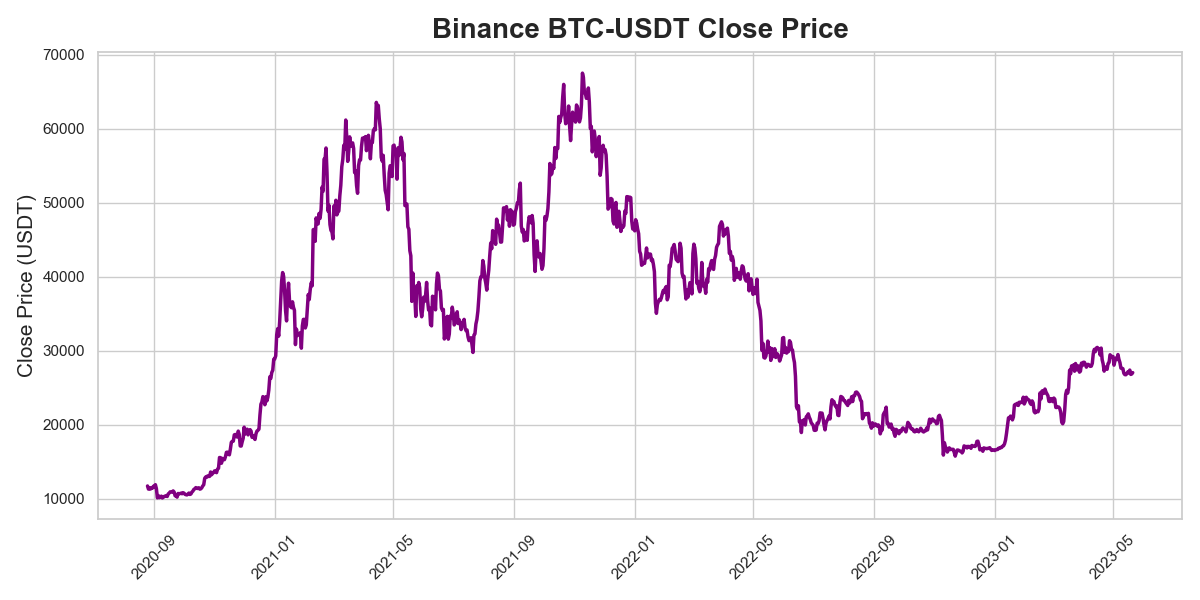
\includegraphics[width=1.0\textwidth]{BTC-USD.png}
        \caption{BTC-USD daily close prices from 23rd August 2020 to 15th May 2023 obtained from Binance. \cite{tradingview}}
        \label{fig:BTC-USD}
    \end{center}
\end{figure}

\begin{figure}[htbp]
    \begin{center}
        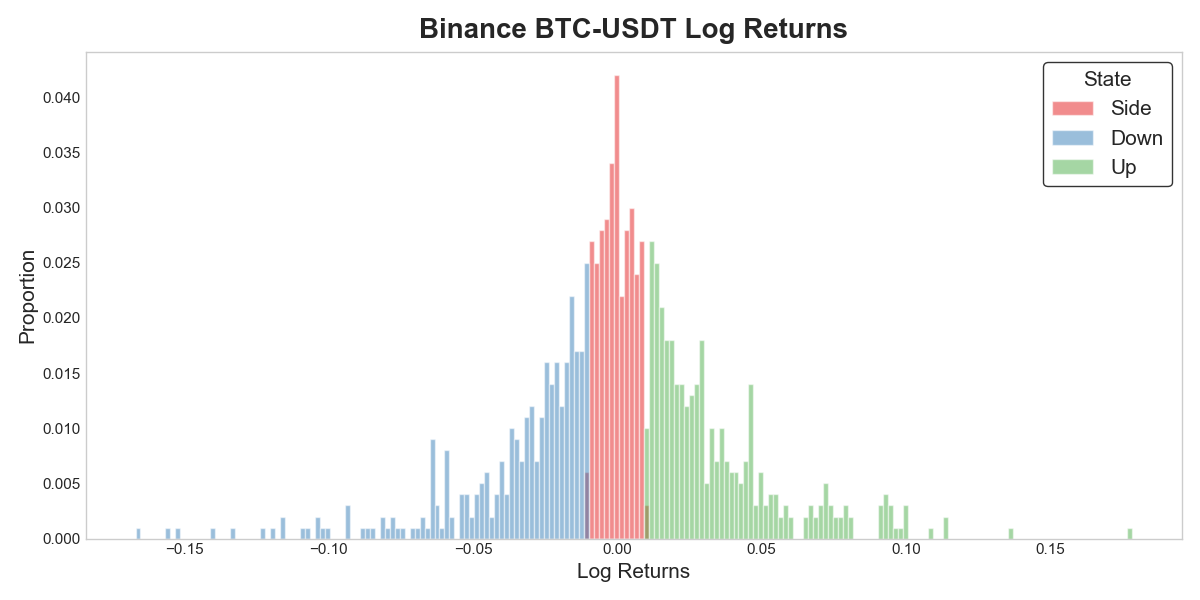
\includegraphics[width=1.0\textwidth]{BTC-USD_hist.png}
        \caption{Distribution of the log returns with respect to predefined market states. \cite{tradingview}}
        \label{fig:BTC-USD-distribution}
    \end{center}
\end{figure}

Observing the distribution of the log-returns of the daily BTC-USDT close price in \ref{fig:BTC-USD-distribution} we may conclude that such a random variable is normally distributed,
given the symmetric property of the distribution with respect to the mean value. Furthermore, it is visible that the kurtosis might be greater than 3,
which implies that the distribution has heavier tails than the normal distribution, i.e. the extreme events are more likely to occur than in the normal distribution.
Such a property is also called {\it leptokurtic} distribution which is a result of the high volatility of the cryptocurrency market.(source?)

Let us now take the ordered sample of states from the BTC-USDT close price time series data and calculate 
the transition and initial probabilities for each state as follows:

\begin{equation}
    A = \begin{pmatrix}
     0.22 & 0.16 & 0.62 \\
     0.32 & 0.27 & 0.41 \\
     0.6 & 0.19 & 0.21 \\
     \end{pmatrix}
     , \quad 
     p= \begin{pmatrix}
     0.4 & 0.19 & 0.41 \\
     \end{pmatrix}
 \end{equation}

where we note that the frequency of observing each state is proportional to the initial distribution $p$, and we assume that state space is $I = \{U,S,D\}$ 
By the definition of the transition matrix $A$, such matrix is also a stochastic matrix since it satisfies the properties given by Equation (1.5).
Each state of the transition matrix $A$ is also non-absorbing since the probability of observing a state $i$ at time $t+1$ given the state $j$ at time $t$ is greater than 0 
and aperiodic since the greatest common divisor of the lengths of all cycles in the chain is 1. Positive recurrence of each state is satisfied as well.
Furthermore, we may also conclude that the state space is irreducible since all states communicate with each other, i.e. there is a non-zero probability of transitioning from any state to any other state.
Therefore, we may conclude that the Markov Chain is ergodic, and the stationary distribution exists, is unique and is approximated by the initial distribution $p$ using Equation \ref{eq:stationary}.
Finally, we may also calculate the expected return time for each state as follows:

\begin{align}
    E[\tau_U(1)|X_0=U] &= \frac{1}{\pi_U} = \frac{1}{0.4} = 2.5 \\
    E[\tau_S(1)|X_0=S] &= \frac{1}{\pi_S} = \frac{1}{0.19} = 5.26 \\
    E[\tau_D(1)|X_0=D] &= \frac{1}{\pi_D} = \frac{1}{0.41} = 2.5
\end{align}

where $\pi$ is the stationary distribution of the Markov Chain. In other words, the expected time of returning to 
state $U$ and $D$ is 2.5 days, and 5.26 days for state $S$. Although, the expected return times provide interesting behavioral insights,
they are simplified by the Markov property of memoryless process, stock and cryptocurrency markets do have certain memory and path-dependence properties as well as they 
are effected by external factors such as news, social media, etc. Therefore, the expected return times are only approximations of the real expected return times.

%********************************** % Third Section  *************************************
\section{Continous-time Markov Chains} 

In the previous section we have considered a discrete-time Markov Chains, i.e. the state space and transition period was discrete. Such period means that 
the chain can stay in a state for integer number of time steps before transitioning to another state. 
For continous-time Markov Chains we will assume that the transition period is continuous, more specifically, the period is exponentially distributed with parameter $\lambda$.

Let us consider a stochastic process $\{X_t,t \geq 0\}$ with a state space $I$ and 
a distribution $\lambda$ such that for all $t \in \mathbb{R}_0^+$ and $i_0,i_1,\ldots,i_{t+1} \in I$ it holds that:

\begin{equation}
P(X_t=j|X_s=i, X_{t_n}=i_n,\ldots,X_{t_1}=i_1) = P(X_t=j|X_s=i)
\end{equation}

where $0 \leq t_1 < \ldots < t_n < s < t $ and so it is trivially seen that such expression is equivalent to the discrete-time Markov Chain property 
given by \ref{DTMC} with the only difference of continuous transition period.

Since the state space remains the same as in discrete-time Markov Chains, we refer to the same transition matrix $A$ and initial distribution $\textbf{p}$.
In upcoming subsection, continuous-time Markov Chain is assumed to be homogeneous, i.e. the transition probabilities are independent of time:

\begin{equation}
p_{i,j}(s,s+t) = p_{i,j}(t), \quad i,j \in I
\end{equation}

which also implies that the transition probability is determined only by the length of the transition period $t$. 
Chapmam Kolmogorov equality for $s,t \geq 0$ also holds for continous-time Markov Chains:

\begin{equation}
p_{i,j}(s+t) = \sum_{k \in I} p_{i,k}(s) p_{k,j}(t), \quad i,j \in I
\end{equation}

Here we also assume that $\lim_{t \to 0_{+}} p_{i,j}(t) = \delta_{i,j}$ where $\delta_{i,j}$ is a Kronecker delta function, 
i.e. the transition probabilities $p_{ij}(t)$ are right continuous at $t=0$. If such condition is satisfied for any homogeneous continous-time Markov Chain, 
then the underlying stochastic process is said to be continuous and there exists its version that is separable, measurable and its trajectories are step functions almost surely. Such version allows us to infer 
certain properties of the stochastic process. 

For example, important property for such Markov Chain given Doob convergence theorem for $s \geq 0$ and $h>0$ is:

\begin{equation}
P(X_t = i, s \leq t \leq s+h|X_s=i) = \exp(-q_ih)
\end{equation}

which means that the probability of staying in state $i$ for time $h$ is equal to $e^{-q_ih}$. 
Non-negative real number $q_{i,j}$ is called {\it transition rate} from state $i$ to state $j$ and absolute transition 
rate $q_i = \sum_{j \neq i} q_{i,j}$ respectively. Trivially, in cases where the transition rate $q_i=0$, the $p_{i,i} = 1$, i.e. the state $i$ is absorbing, 
once the chain enters such state it remains in such state for infinite amount of time. On the contrary, if $0 < q_i < \infty$ then the state $i$ is non-absorbing and stable, therefore
the chain will eventually leave such a state. For infinite transition rate $q_i = \infty$ the state $i$ is called {\it unstable} where the time of staying in such state is almost surely zero.

If we consider a stable state $i$ then its expected time of staying in such state is exponentially 
distributed with expected value of $1/q_i$. In other words, the expected time of staying in state $i$ is equal 
to the inverse of the transition rate $q_i$.

Since, we have already defined that the process has exponentially distributed transition period, we may define a {\it holding time} $T_i$ as a random variable that denotes the time of staying in state $i$:

\begin{equation}
T_i = \inf \{t \geq 0 : X_t \neq i | X_0 = i\}
\end{equation}

from which it follows that $P(T_i>s) = P(X_t=i,0 \leq t \leq s|X_0=i) = e^{-q_i s}$ and its probability density functions is:

\begin{equation}
    f(x) = 
    \begin{cases}
        q_i e^{-q_i x}, & x \geq 0\\
        0, & \text{elsewhere}
    \end{cases}
\end{equation}

% is homogeneous, we may define a transition matrix $Q$ as a matrix of transition rates between each state $i,j \in I$ such that:
According to the properties of the transition rates, such time-homogeneous continuous Markov Chain should satisfy following equations:
\begin{equation}
    \begin{aligned}
    P(X_{t+h}=i|X_t=i) &= 1 - q_i h + o(h) \\
    P(X_{t+h}=j|X_t=i) &= q_{i,j} h + o(h), \quad i \neq j
    \end{aligned}
\end{equation}

where $o(h)$ is a function of $h$ such that $\lim_{h \to 0} \frac{o(h)}{h} = 0$. Let us denote $\textbf{Q}$ as transition rates matrix with entries $\{q_{i,j}: i,j \in I\}$.

Non-negative real number $q_{i,j}$ is called {\it transition rate} from state $i$ to state $j$ and absolute transition

Such intensities resemble the probability functions of Poisson process,
 and indeed homogeneous continous-time Markov Chain is a special case of Poisson process with intensity $\lambda \geq 0$ if following conditions are satisfied:

\begin{itemize}
\item [1)] Stochastic process is viewed as a jump process, i.e. current state $i$ either stays in state $i$ or jumps to another state $j=i+1$. Therefore, given an interval $[t,t+h]$ the probability of jumping to another state is $\lambda h + o(h)$ and the probability of staying in state $i$ is $1-\lambda h + o(h)$.
\item [2)] Intensity $\lambda$ is constant, i.e. the probability of jumping to another state is independent of time, i.e. depends only on the length of the interval. We refer to such process as homogeneous Poisson process.
\item [3)] Number of jumps in disjoint intervals are independent, i.e. the probability of jumping to another state in disjoint intervals $[t_1,t_1+h]$ and $[t_2,t_2+h]$ is equal to the probability of jumping to another state in interval $[t_1,t_1+h] \cup [t_2,t_2+h]$.
\item [4)] The probability of more than one jump in a sufficiently small interval is negligible, i.e. the probability of jumping to another state in interval $[t,t+h]$ is $o(h)$.
\item [5)] Process starts in state $i=0$ at time $t=0$.
\end{itemize}

In a case of constant return rates, the matrix $\textbf{Q}$ with entries $q_{i} = - \lambda$ and $q_{i,j} = \lambda$ as follows:

\begin{equation}
    \textbf{Q} = 
    \begin{pmatrix}
    -\lambda & \lambda & 0 & 0 & \ldots \\
    0 & -\lambda & \lambda & 0 & \ldots \\
    0 & 0 & -\lambda & \lambda & \ldots \\
    \vdots & \vdots & \vdots & \vdots & \ddots \\
    \end{pmatrix}
\end{equation}

\subsection{Cryptocurrency market movements II.}

\section{Hidden Markov Model}

Up until now we have considered visible states in a sense that the sequence of states was known, we refer to these models as $visible$ $Markov$ $Models$. In this section we will consider a situation in which we do not observe the states directly but only as a guess given other visible observations that are available to us. These "visible" observations are considered as an emissions from the hidden state sequence. Thus, the observations are assumed to be generated by the hidden states. We may interpret this relation by the following diagram where we have a hidden state sequence $Z = \{z_1,z_2,\ldots,z_T\}$:

\begin{figure}[htbp]
\begin{center}
\begin{tikzpicture}[]
% states
\node[state] (s1) at (0,2) {$z_1$}
    edge [loop above]  ();
\node[state] (s2) at (2,2) {$z_2$}
    edge [<-,bend right=45] node[auto,swap] {$a_{12}$} (s1)
    edge [->,bend left=45] (s1)
    edge [loop above] ();
\node[state] (s3) at (4,2) {$z_3$}
    edge [<-,bend right=45] node[auto,swap] {$a_{23}$} (s2)
    edge [->,bend left=45] (s2)
    edge [loop above] ();
\node[state] (s4) at (6,2) {$z_4$}
    edge [<-,bend right=45] node[auto,swap] {$a_{34}$}  (s3)
    edge [->,bend left=45] (s3)
    edge [loop above] ();
% observations
\node[observation] (y1) at (2,0) {$x_1$}
    edge [lightedge] node[auto,swap] {$b_1(x_1)$} (s1)
    edge [lightedge] (s2)
    edge [lightedge] (s3)
    edge [lightedge] (s4);
\node[observation] (y2) at (4,0) {$x_2$}
    edge [lightedge] (s1)
    edge [lightedge] (s2)
    edge [lightedge] (s3)
    edge [lightedge] node[auto,swap] {$b_4(x_2)$} (s4);
\end{tikzpicture}
\end{center}
\caption{An HMM with 4 hidden states which emits 2 discrete observable states denoted by $x_1$ or $x_2$.
$a_{ij}$ is the probability to transition from state $z_i$ to state $z_j$.
$b_j(x_k)$ is the probability to emit symbol $x_k$ in state $z_j$.}
\end{figure}

There are 3 main assumptions of Hidden Markov Models as a consequence of the properties of Markov processes. For $Z = \{z_t\}_{t=0}^T$ being the hidden state sequence:

\begin{itemize}
\item[1)] The Markov assumption - this assumption states that the next hidden state $z_{t+1}$ depends only on the current state $z_t$, so that the transition probabilities are defined as:

\begin{equation}
P(z_{t+1} = j| z_{t} = i,z_{t-1} = l,\ldots,z_{0} = n) = P(z_{t+1} = j| z_{t} = i) = p_{ij}
\end{equation}

It it also possible to assume that the states in HMM are dependent beyond the current state therefore giving rise to k-order HMMs as opposed to classical first-order HMM, moreover, such variations are uneasy to analyse.

\item[2)] The stationary assumption - The transition matrix is invariant of the time, thus for any arbitrarily set time $t_1$ and $t_2$:

\begin{equation}
P(z_{t_1+1} = j| z_{t_1}) = P(z_{t_2+1} = j| z_{t_2} = i) = p_{ij}
\end{equation}

\item[3)] The observation independence assumption - The current observation or output is statistically independent of the previous observations. So if we have a observation sequence $X = \{x_1,x_2,\ldots,x_T\}$ then:

\begin{equation}
P(X|z_1,z_2,\ldots,z_T, \lambda) = \prod_{t=1}^T P(x_t|z_t,\lambda)
\end{equation}

\end{itemize}

Given these assumptions we define the joint probability of the hidden states and the observations $P(X,Z)$ as follows:

\begin{equation}
P(X, Z) = \prod_{t=1}^T P(z_t|z_{t-1}) P(x_t|z_t)
\end{equation}



There are mainly 3 fundamental problems in HMM that need to be resolved as in (Oliver C. Ibe):

\begin{itemize}
\item[1.] Evaluation problem - Given a model denoted as $\lambda = (P,\theta,\pi)$ and an observation sequence $X = x_1, x_2,\ldots,x_T$, how to efficiently compute the probability that the model generated the observation sequence, in other words, what is $P(X|\lambda)$? 
\item[2.] Decoding problem - Given a model $\lambda = (P,\theta,\pi)$, what is the most likely sequence of hidden states that could have generated a given observation sequence? Thus we would like to find $Z = \underset{Z}{\arg\max} P(Z,X|\lambda)$, where $Z$ is the hidden state sequence. 
\item[3.] The learning problem - Given a set of observation sequences find the HMM that best explains the observation sequence. Thus, find the values of $\lambda$ that maximise $P(X|\lambda)$ or in order to estimate the most likely parameters of HMM for a given observation sequence. 
\end{itemize}

The most traditional approaches in solving these 3 fundamental problems differ and one may not suffice in solving all three. The evaluation problem is usually by forward-backward algorithm, the decoding problem by well-known Viterbi algorithm and the last learning problem by Baum-Welsch algorithm which is a special case of Expectation-maximization (EM) algorithm. 

\subsection{Forward and Backward algorithm}

While given a sequence of observations, in our case observable states, denoted by $X = x_1,x_2,\ldots,x_T$ and a model $\lambda = (P,\theta,\pi)$ we wold like to compute the conditional probability of observing the sequence $X$ under the model constraints. Thus:

 \begin{equation}
P(X| \lambda) = \sum_Z P(X|Z,\lambda)*P(Z|\lambda)
\end{equation}

where $Z = z_1,z_2,\ldots,z_T$ is a fixed sequence of hidden states. Our goal may be divided into two parts while the first part $P(X|Z,\lambda)$ computes the conditional probability of the observation sequence X given the sequence Z and model $\lambda$ and the second part $P(Z|\lambda)$ accounts only for the transition probabilities among the hidden states. To summarise:

\begin{align}
P(X| Z, \lambda) &= \prod_{t=1}^T  P(x_t|z_t,\lambda) = \theta_{z_1}(x_1) \prod_{t=2}^T \theta_{z_t}(x_t) \\ \nonumber
P(Z|\lambda)&= \pi_{z_1} * \prod_{t=2}^{T} p_{z_t z_{t+1}}
\end{align}

where $\theta_{z_t}(x_t)$ is the emission probability from observation $x_t$ into $z_t$ in our model and $p_{z_t z_{t+1}}$ are the transition probabilities for the given sequence Z. After substitution of terms from Eq. 1.8 into Eq 1.7 we obtain:

\begin{align}
P(X| \lambda) &= \sum_Z P(X|Z,\lambda)*P(Z|\lambda) \\ \nonumber
&= \sum_{z_1,\ldots,z_T}\theta_{z_1}(x_1) \pi_{z_1} \prod_{t=2}^{T} p_{z_t z_{t+1}} \theta_{z_t}(x_t)
\end{align}

The summation above refers to all possible permutations of the sequence of hidden states Z which implies that we would have $N^T$ possible sequences if we assume that $N$ indicates all possible hidden states at each step. Furthermore, in order to calculate $P(X|\lambda)$ we have $2TN^T$ calculations which is exponential in T and not feasible for real application. As opposed to brute-force procedure as described above we take use of a forward and backward algorithm. 

\subsubsection{Forward algorithm}

Previous introduction required huge amounts of calculations that were essentially unnecessary, redundant. Each sequence can be decomposed into multiple subsequences which are shared among different sequences and do not need to be recomputed again. These subsequences can be represented by a trellis as shown in Fig 1.2. With a help of such diagram we may imagine recording the probability of each distinct subsequence at each time step. In other words, we wish to compute the joint probability $P(z_t,x_1,x_2,\ldots,x_t)$ while taking advantage of the conditional independence of $x_t$ which only depends on $z_t$, moreover, due to Markov assumption, $z_t$ depends only on $z_{t-1}$. Let us now define the forward probability variable $\alpha_t(i)$ as follows:

 \begin{equation}
\alpha_t(i) = P(x_1,x_2,\ldots,x_{t-1},x_t,z_t=i |\lambda)
\end{equation}

Which we may also define as the probability of being in state i at time t after having observed the sequence ${x_1,x_2,\ldots,x_t}$. The calculation therefore results in summing the incoming arcs at trellis node which is derived from:

\begin{align}
\alpha_t(i) &= P(x_1,x_2,\ldots,x_{t-1},x_t,z_t=i |\lambda) \\ \nonumber
&= P(x_t|z_t=I, \lambda) P(x_1,x_2,\ldots,x_{t-1},z_t=i |\lambda)  \\ \nonumber
&= P(x_t|z_t=i, \lambda) \sum_{j \in I} P(z_t = I| z_{t-1}=j,\lambda) P(x_1,x_2,\ldots,x_{t-1},z_{t-1}=j |\lambda) \\ \nonumber
&= \theta_i(x_t) \sum_{j=1}^N p_{ji} \alpha_{t-1}(j)
\end{align}

Where $I$ is a set of all possible hidden states, $i,j$ denote elements of $I$ and $N$ the size of set $|I|$. We would repeat the iterative procedure until the termination at time T where $P(X|\lambda) = \sum_{i=1}^N  \alpha_T(i) = \sum_{i=1}^N P(X,z_T=I|\lambda)$. Moreover, we initialise the trellis with $\alpha_1(i)=\pi_i \theta_i(x_1)$. Resulting algorithm requires time complexity of $O(TN^2)$ which is a significant improvement from the brute force approach with complexity of $O(2TN^T)$.
  
\begin{figure}[htbp]
\begin{center}
\begin{tikzpicture}[]
% 1st column
\node               at (0,6) {$t=1$};
\node[state] (s1_1) at (0,5) {$z_1$};
\node[mainstate] (s2_1) at (0,4) {$z_2$};
\node[state] (s3_1) at (0,3) {$\ldots$};
\node[state] (s4_1) at (0,2) {$z_N$};
\node at (0,1) {$x_1$};
% 2nd column
\node               at (2,6) {$t=2$};
\node[mainstate] (s1_2) at (2,5) {$z_1$}
    edge[lightedge] (s1_1)
    edge[lightedge] (s2_1)
    edge[lightedge] (s3_1)
    edge[lightedge] (s4_1);
\node[state] (s2_2) at (2,4) {$z_2$}
    edge[lightedge] (s1_1)
    edge[lightedge] (s2_1)
    edge[lightedge] (s3_1)
    edge[lightedge] (s4_1);
\node[state] (s3_2) at (2,3) {$\ldots$}
    edge[lightedge] (s1_1)
    edge[lightedge] (s2_1)
    edge[lightedge] (s3_1)
    edge[lightedge] (s4_1);
\node[state] (s4_2) at (2,2) {$z_N$}
    edge[lightedge] (s1_1)
    edge[lightedge] (s2_1)
    edge[lightedge] (s3_1)
    edge[lightedge] (s4_1);
\node at (2,1) {$x_2$};
% 3rd column
\node               at (4,6) {$t=3$};
\node[mainstate] (s1_3) at (4,5) {$z_1$}
    edge[lightedge]  (s1_2)
    edge[lightedge] (s2_2)
    edge[lightedge] (s3_2)
    edge[lightedge] (s4_2);
\node[state] (s2_3) at (4,4) {$z_2$}
    edge[lightedge] (s1_2)
    edge[lightedge] (s2_2)
    edge[lightedge] (s3_2)
    edge[lightedge] (s4_2);
\node[state] (s3_3) at (4,3) {$\ldots$}
    edge[lightedge] (s1_2)
    edge[lightedge] (s2_2)
    edge[lightedge] (s3_2)
    edge[lightedge] (s4_2);
\node[state] (s4_3) at (4,2) {$z_N$}
    edge[lightedge] (s1_2)
    edge[lightedge] (s2_2)
    edge[lightedge] (s3_2)
    edge[lightedge] (s4_2);
\node at (4,1) {$x_3$};
% 4th column
\node               at (6,6) {$t=4$};
\node[mainstate] (s1_4) at (6,5) {$z_1$}
    edge[lightedge]  (s1_3)
    edge[lightedge] (s2_3)
    edge[lightedge] (s3_3)
    edge[lightedge] (s4_3);
\node[state] (s2_4) at (6,4) {$z_2$}
    edge[lightedge] (s1_3)
    edge[lightedge] (s2_3)
    edge[lightedge] (s3_3)
    edge[lightedge] (s4_3);
\node[state] (s3_4) at (6,3) {$\ldots$}
    edge[lightedge] (s1_3)
    edge[lightedge] (s2_3)
    edge[lightedge] (s3_3)
    edge[lightedge] (s4_3);
\node[state] (s4_4) at (6,2) {$z_N$}
    edge[lightedge] (s1_3)
    edge[lightedge] (s2_3)
    edge[lightedge] (s3_3)
    edge[lightedge] (s4_3);
\node at (6,1) {$x_4$};
% 5th column
\node               at (8,6) {$t=5$};
\node[mainstate] (s1_5) at (8,5) {$z_1$}
    edge[lightedge]  (s1_4)
    edge[lightedge] (s2_4)
    edge[lightedge] (s3_4)
    edge[lightedge] (s4_4);
\node[state] (s2_5) at (8,4) {$z_2$}
    edge[lightedge] (s1_4)
    edge[lightedge] (s2_4)
    edge[lightedge] (s3_4)
    edge[lightedge] (s4_4);
\node[state] (s3_5) at (8,3) {$\ldots$}
    edge[lightedge] (s1_4)
    edge[lightedge] (s2_4)
    edge[lightedge] (s3_4)
    edge[lightedge] (s4_4);
\node[state] (s4_5) at (8,2) {$z_N$}
    edge[lightedge] (s1_4)
    edge[lightedge] (s2_4)
    edge[lightedge] (s3_4)
    edge[lightedge] (s4_4);
\node at (8,1) {$x_5$};
\end{tikzpicture}
\end{center}
\caption{Trellis of the observation sequence $x_1$,\ldots,$x_5$ for the above HMM.\@ As an example, the transition between state $z_1$ at time t=2 and state $z_4$ at time t=3 has probability $\alpha_2(z_1)p_{14}\theta_{z_4}(x_3)$, where $\alpha_t(i)$ is the probability to be instate $i$ at time t.}
\end{figure}

\pagebreak

\subsubsection{Backward algorithm}

While computing the backward probability variable denoted as $\beta_t(i)$ we assume the reversed iterative procedure. Let us define the backward probability variable as:

\begin{align}
\beta_t(i) &= P(x_{t+1},x_{t+2},\ldots,x_{t-1},x_t|z_t=i ,\lambda) \\ \nonumber
&= \sum_{i,j \in I} P(x_{t+1},x_{t+2},\ldots,x_{t-1},x_t,z_{t+1}=j|z_t=i ,\lambda)   \\ \nonumber
&= \sum_{i,j \in I} P(x_{t+1}|z_{t+1}=j) P(x_{t+2},\ldots,x_{t-1},x_t|z_{t+1}=j) P(z_{t+1}=j|z_{t}=i,\lambda) \\ \nonumber
&= \sum_{j=1}^N \theta_j(x_{t+1})p_{ij} \beta_{t+1}(j)
\end{align}

As we could have in forward algorithm we define effectively 3 steps:

\begin{itemize}
\item[1.] Initialization step: with default value of $\beta_T(i) = 1$ for $i \in {1,2,\ldots,N}$. 
\item[2.] Induction step: 

\begin{equation}
\beta_t(i) = \theta_j(x_{t+1})p_{ij} \beta_{t+1}(j)
\end{equation}

Afterwards, we update the time t = t-1 and check whether expression above holds which is as long as t $>$ 0.
\item[3.] Termination step: once the iterative procedure is exhausted, i.e.\ when t=0 we have the estimate of $P(X|\lambda)$ as:

\begin{equation}
P(X|\lambda) = \sum_{j=1}^N \theta_j(x_{1})\pi_{i} \beta_{1}(i) = \sum_{j=1}^N \alpha_1(i)  \beta_{1}(i)
\end{equation}

\end{itemize}

Getting everything together we may prove that the forward and backward algorithms coincide in solving the posterior joint and marginal distributions of all hidden states. Consider the case of posterior joint distribution:

\begin{align}
P(X|\lambda) &= \sum_{i=1}^N P(X,z_t=i|\lambda) \\ \nonumber
&= \sum_{i=1}^N P(x_1,x_2,\ldots,x_{t},x_{t+1},\ldots,x_{T}|z_t=i,\lambda) P(z_t = i|\lambda) \\ \nonumber
&= \sum_{i=1}^N P(x_1,x_2,\ldots,x_{t}|z_t=i,\lambda) P(x_{t+1},\ldots,x_{T}|z_t=i,\lambda) P(z_t = i|\lambda) \\ \nonumber
&= \sum_{i=1}^N P(x_1,x_2,\ldots,x_{t},z_t=i|\lambda) P(x_{t+1},\ldots,x_{T}|z_t=i,\lambda) \\ \nonumber
&= \sum_{i=1}^N \alpha_{t}(i) \beta_t(i) 
\end{align}

See that above we take a use of conditional independence of observations given the hidden state and therefore we may transform the problem using already known variables for forward and backward passes over the hidden states. Thus, the posterior marginal distribution is:

\begin{equation}
P(X, z_t=i|\lambda) = \alpha_t(i) \beta_t(i)
\end{equation}

\subsection{Viterbi algorithm}

Once we solve the evaluation problem, thus finding the optimal procedure in computing the posterior marginal distributions of all hidden states and $P(X|\lambda)$, we may visualise the result in a trellis as shown in Figure 1.2. The second problem, decoding problem, aims to find the sequence of hidden states $Z^*$ that most likely produced observation sequence $X$. Finding the most likely sequence $Z^*$ maximazes $P(Z|X,\lambda)$. As in the encoding problem, the complexity of the optimisation problem explodes if we decide to compute all possible sequences of hidden states to $N^T$ calculations. The solution as in the forward and backward algorithm simplifies when we calculate the hidden state with highest probability individually rather than entire sequence up to time $t$. The idea is that once we find the most likely hidden state given observation and the model at each time step we may discard the rest of the possible hidden states since they obviously could not have most likely produced the observation. The complexity of the optimal sequence of hidden states decreases significantly to $NT$ thus transforming the exponential complexity into linear. As in forward and backward algorithm we define variable $\gamma_t(i)$ as:

\begin{equation}
\gamma_t(i) = P(z_t=i|X,\lambda) = \frac{P(X,z_t=i|\lambda)}{P(X|\lambda)} =\frac{\alpha_t(i) \beta_t(i)}{\sum_{i=1}^N \alpha_t(i) \beta_t(i)} \propto \alpha_t(i) \beta_t(i)
\end{equation}

Where the expressions in the third equality are obtained as a solution to a before mentioned equations. Also, the $P(X|\lambda)$ serves only as a normalising constant and is irrelevant for the optimisation given the respective time step. Moreover, the conditional probability $\gamma_t(i)$ forms a conditional probability mass function since it is non-negative for all possible values of hidden states and observations and the sum over all possible hidden states at each time step is:

\begin{equation}
\sum_{i=1}^N  \gamma_t(i) = 1
\end{equation}

This would be one of the possible ways to estimate the most likely hidden states individually and then combine them sequentially to obtain the whole sequence of hidden states as:

\begin{equation}
z_t^* = \underset{i \in I}{\arg\max} \{\gamma_t(i)\}
\end{equation}

Method as described by the Eq 1.17 and 1.19 is also called maximum a posteriori probability estimate (hereinafter `MAP estimate`) which equals to the mode of the posterior distribution. If the posterior distribution is discrete, the mode is simply the value of a random variable with the highest probability. For continuous distributions the mode is a value of a random variable for which the likelihood/log-likelihood function attains its local maximum/maxima. Assuming now $Z$ denotes the continuous random variable of hidden states and observation sequence $X$ up to time t is present, the MAP estimate of the hidden state $\hat{Z}_{MAP}$ at a given point in time is:

\begin{align}
\hat{z}_{t,MAP} &= \underset{z_t}{\arg\max} \: f(Z_t|X) \\ \nonumber
&= \underset{z_t}{\arg\max} \: \frac{f(X|Z_t)g(Z_t)}{\int_{I} f(X|Z_t)g(Z_t) \,dZ} \\ \nonumber
&= \underset{z_t}{\arg\max} \: f(X|Z_t)g(Z_t)\\ \nonumber
\end{align}

Where $g$ indicates probability density function of $Z_t$, so called prior distribution, and $I$ is its domain. The second equality follows from the Bayes' Theorem. The result clearly holds for the discrete case:

\begin{align}
\hat{z}_{t,MAP} &= \underset{z_t}{\arg\max} \: P(Z_t=i|X) \\ \nonumber
&= \underset{z_t}{\arg\max} \: \frac{P(X|Z_t=i)P(Z_t=i)}{\sum_{i=1}^N P(X|Z_t=i)P(Z_t=i)} \\ \nonumber
&= \underset{z_t}{\arg\max} \:P(X|Z_t=i)P(Z_t=i)\\ \nonumber
&= z_t^*\\ \nonumber
\end{align}

However, the solution as such might not produce the most likely sequence of states given the sequence of observations. This is due to the fact that the individual estimates do not incorporate the transition probability between most likely states at time t-1 and t. Hence, it might be possible that some states are highly unlikely to transition into other that were evaluated as most likely. Fortunately, the mentioned shortcomings of such approach are easily solved by Viterbi algorithm.

In order to find the most likely sequence of hidden states $Z^*={z_1^*,z_2^*,\ldots,z_T^*}$ given the observation sequence $X={x_1,x_2,\ldots,x_T}$ it is necessary to maximise with respect to the whole sequence rather than individually to avoid less likely transitions as introduced. The algorithm therefore defines a variable as follows:

\begin{equation}
\delta_t(i) = \underset{Z_{t-1}}{\max}\:P(z_1,z_2,\ldots,z_t=i,x_1,x_2,\ldots,x_{t-1},x_{t}|\lambda)
\end{equation}

That is the most likely state sequence given the observation sequence up to time $t$. Moreover, for the purpose of the algorithm we also define variable $\psi_t(i)$ that stores the node of the incoming arc that leads to the most probable state path.

\begin{equation}
\psi_t(j) = \underset{i \in I}{\arg\max} \: \delta_{t-1}(i)p_{ij}
\end{equation}

\vspace{0.3cm}

\noindent
Then we can easily provide the steps to obtain the most likely state sequence:

\begin{itemize}
\item[1.] Initialize the algorithm given the initial distribution of hidden states $\pi$:

\begin{align}
\delta_1(i) &= \pi_i b_i(o_1)  \\
\psi_1(i)& = 0
\end{align}

where we compute the initial values of above variables for each hidden state $i \in I$.

\item[2.] Recursive step:

\begin{align}
\delta_1(i) &= \underset{i \in I}{\arg\max} \: \delta_{t-1}(i)p_{ij} b_j(o_t)  \\
\psi_t(j)& = \underset{i \in I}{\arg\max} \: \delta_{t-1}(i)p_{ij}
\end{align}

At each iterative step we update the time so that $t=t+1$. The second step continues as long as the $t<T$ if that does not hold the third step terminates the algorithm and we backtrack the most likely state sequence. Although, recursive step is very similar to the induction step in the forward algorithm there exist a main difference between the two that lies in the fact that Viterbi algorithm uses maximization instead of summation over previous states. 

\item[3.] Termination step for the last observation 

\begin{align}
P^* &= \underset{i \in I}{\max} \: \delta_{T}(i) \\
q_T^* & = \underset{i \in I}{\arg\max} \: \delta_{T}(i)
\end{align}

\item[4.] Backtrack the optimal state sequence:

\begin{equation}
z_t^* = \psi_{t+1}(z_{t+1}^*)
\end{equation}

For $t = T-1,T-2,\ldots,1$.

\end{itemize}

The resulting most likely state path can be visually viewed as in the form of a path within the trellis introduced in Fig. 1.2:

\begin{figure}[htbp]
\begin{center}
\begin{tikzpicture}[]
% 1st column
\node               at (0,6) {$t=1$};
\node[state] (s1_1) at (0,5) {$z_1$};
\node[mainstate] (s2_1) at (0,4) {$z_2$};
\node[state] (s3_1) at (0,3) {$\ldots$};
\node[state] (s4_1) at (0,2) {$z_N$};
\node at (0,1) {$x_1$};
% 2nd column
\node               at (2,6) {$t=2$};
\node[mainstate] (s1_2) at (2,5) {$z_1$}
    edge[lightedge] (s1_1)
    edge[lightedge] (s2_1)
    edge[lightedge] (s3_1)
    edge[lightedge] (s4_1);
\node[state] (s2_2) at (2,4) {$z_2$}
    edge[lightedge] (s1_1)
    edge[lightedge] (s2_1)
    edge[lightedge] (s3_1)
    edge[lightedge] (s4_1);
\node[state] (s3_2) at (2,3) {$\ldots$}
    edge[lightedge] (s1_1)
    edge[mainedge] (s2_1)
    edge[lightedge] (s3_1)
    edge[lightedge] (s4_1);
\node[state] (s4_2) at (2,2) {$z_N$}
    edge[lightedge] (s1_1)
    edge[lightedge] (s2_1)
    edge[lightedge] (s3_1)
    edge[lightedge] (s4_1);
\node at (2,1) {$x_2$};
% 3rd column
\node               at (4,6) {$t=3$};
\node[mainstate] (s1_3) at (4,5) {$z_1$}
    edge[lightedge]  (s1_2)
    edge[lightedge] (s2_2)
    edge[mainedge] (s3_2)
    edge[lightedge] (s4_2);
\node[state] (s2_3) at (4,4) {$z_2$}
    edge[lightedge] (s1_2)
    edge[lightedge] (s2_2)
    edge[lightedge] (s3_2)
    edge[lightedge] (s4_2);
\node[state] (s3_3) at (4,3) {$\ldots$}
    edge[lightedge] (s1_2)
    edge[lightedge] (s2_2)
    edge[lightedge] (s3_2)
    edge[lightedge] (s4_2);
\node[state] (s4_3) at (4,2) {$z_N$}
    edge[lightedge] (s1_2)
    edge[lightedge] (s2_2)
    edge[lightedge] (s3_2)
    edge[lightedge] (s4_2);
\node at (4,1) {$x_3$};
% 4th column
\node               at (6,6) {$t=4$};
\node[mainstate] (s1_4) at (6,5) {$z_1$}
    edge[mainedge]  (s1_3)
    edge[lightedge] (s2_3)
    edge[lightedge] (s3_3)
    edge[lightedge] (s4_3);
\node[state] (s2_4) at (6,4) {$z_2$}
    edge[lightedge] (s1_3)
    edge[lightedge] (s2_3)
    edge[lightedge] (s3_3)
    edge[lightedge] (s4_3);
\node[state] (s3_4) at (6,3) {$\ldots$}
    edge[lightedge] (s1_3)
    edge[lightedge] (s2_3)
    edge[lightedge] (s3_3)
    edge[lightedge] (s4_3);
\node[state] (s4_4) at (6,2) {$z_N$}
    edge[lightedge] (s1_3)
    edge[lightedge] (s2_3)
    edge[lightedge] (s3_3)
    edge[lightedge] (s4_3);
\node at (6,1) {$x_4$};
% 5th column
\node               at (8,6) {$t=5$};
\node[mainstate] (s1_5) at (8,5) {$z_1$}
    edge[lightedge]  (s1_4)
    edge[lightedge] (s2_4)
    edge[lightedge] (s3_4)
    edge[lightedge] (s4_4);
\node[state] (s2_5) at (8,4) {$z_2$}
    edge[mainedge] (s1_4)
    edge[lightedge] (s2_4)
    edge[lightedge] (s3_4)
    edge[lightedge] (s4_4);
\node[state] (s3_5) at (8,3) {$\ldots$}
    edge[lightedge] (s1_4)
    edge[lightedge] (s2_4)
    edge[lightedge] (s3_4)
    edge[lightedge] (s4_4);
\node[state] (s4_5) at (8,2) {$z_N$}
    edge[lightedge] (s1_4)
    edge[lightedge] (s2_4)
    edge[lightedge] (s3_4)
    edge[lightedge] (s4_4);
\node at (8,1) {$x_5$};
\end{tikzpicture}
\end{center}
\caption{Trellis of the observation sequence $x_1$,\ldots,$x_5$ for the HMM.\@ Bold lines illustrate the most likely sequence found by the Viterbi algorithm.}
\end{figure}


\newpage


\section{Kalman Filters}




\nomenclature[z-DEM]{DEM}{Discrete Element Method}
\nomenclature[z-FEM]{FEM}{Finite Element Method}
\nomenclature[z-PFEM]{PFEM}{Particle Finite Element Method}
\nomenclature[z-FVM]{FVM}{Finite Volume Method}
\nomenclature[z-BEM]{BEM}{Boundary Element Method}
\nomenclature[z-MPM]{MPM}{Material Point Method}
\nomenclature[z-LBM]{LBM}{Lattice Boltzmann Method}
\nomenclature[z-MRT]{MRT}{Multi-Relaxation Time}
\nomenclature[z-RVE]{RVE}{Representative Elemental Volume}
\nomenclature[z-GPU]{GPU}{Graphics Processing Unit}
\nomenclature[z-SH]{SH}{Savage Hutter}
\nomenclature[z-CFD]{CFD}{Computational Fluid Dynamics}
\nomenclature[z-LES]{LES}{Large Eddy Simulation}
\nomenclature[z-FLOP]{FLOP}{Floating Point Operations}
\nomenclature[z-ALU]{ALU}{Arithmetic Logic Unit}
\nomenclature[z-FPU]{FPU}{Floating Point Unit}
\nomenclature[z-SM]{SM}{Streaming Multiprocessors}
\nomenclature[z-PCI]{PCI}{Peripheral Component Interconnect}
\nomenclature[z-CK]{CK}{Carman - Kozeny}
\nomenclature[z-CD]{CD}{Contact Dynamics}
\nomenclature[z-DNS]{DNS}{Direct Numerical Simulation}
\nomenclature[z-EFG]{EFG}{Element-Free Galerkin}
\nomenclature[z-PIC]{PIC}{Particle-in-cell}
\nomenclature[z-USF]{USF}{Update Stress First}
\nomenclature[z-USL]{USL}{Update Stress Last}
\nomenclature[s-crit]{crit}{Critical state}
\nomenclature[z-DKT]{DKT}{Draft Kiss Tumble}
\nomenclature[z-PPC]{PPC}{Particles per cell}
%!TEX root = ../thesis.tex


\if pdf
    \graphicspath{{Chapter4/Figs/Raster/}{Chapter4/Figs/PDF/}{Chapter4/Figs/}}
\else
    \graphicspath{{Chapter4/Figs/Vector/}{Chapter4/Figs/}}
\fi

\chapter{Hidden Markov Models}

Until now, we have considered visible states in a sense that the sequence of states was known, we refer to these models as \textit{visible Markov Models}.
In this section we will consider a situation in which we do not observe the states directly but only as a "guess" given other visible observations that are available to us. 
These "visible" observations are labeled as emissions emitted by the respective hidden state. Thus, the observations are assumed to be generated by certain hidden stochastic process, i.e. a Markov Chain.\footnote{Models that
comprise unobserved random variables, e.g. Hidden Markov Models, are called \textbf{latent variable models}, \textbf{missing data models}, or also \textbf{models with incomplete data}}
In general, we could assume that the state and emission space is not necessarily finite, but we will follow the classical definition by \cite{Rabiner1989} and \cite{Elliott1995} of Hidden Markov Models and assume that at least state space is finite.

\section{Discrete Hidden Markov Model}

Revisiting previous section, we have defined a transition matrix $\textbf{A}$ and initial distribution $\textbf{p}$ for a homogeneous Markov Chain. Both of these parameters are used to describe the hidden stochastic process.
In order to describe the emissions, we will define an $N \times M$ \textit{emission matrix} $\textbf{B}$\footnote{Also referred to as \textbf{observation matrix} and \textbf{observations} respectively} as follows:

\begin{equation}
    \textbf{B} = \begin{pmatrix}
    b_1(y_1) & b_1(y_2) & \ldots & b_1(y_M) \\
    b_2(y_1) & b_2(y_2) & \ldots & b_2(y_M) \\
    \vdots & \vdots & \ddots & \vdots \\
    b_N(y_1) & b_N(y_2) & \ldots & b_N(y_M) \\
    \end{pmatrix}
\end{equation}

\noindent where $N$ represents number of states and $M$ number of possible emission symbols.

Probabilistically each element of the matrix represents conditional probability of emitting symbol $k$ for all $k = 1,2,\ldots,M$, given state $i$: 

\begin{equation}
    b_{i}(k) = \mathbb{P}(Y_t = k|X_t = i) 
\end{equation}

As stated at the beginning of this section, observer does not have access to the hidden states, but only to the emissions emitted by the hidden states. 
Thus, observing only another stochastic process $\{Y_t, t \in \mathbb{N}_0\}$ linked to hidden Markov Chain s.t. it governs the distribution of $Y_t$. 
In other words, entire statistical inference, even in terms of the hidden Markov process, is based on the observed sequence of emissions $\{Y_t\}$.

Considering the discrete time index $t$, Hidden Markov model is bivariate discrete-time stochastic process $\{X_t,Y_t\}$, where $\{Y_t\}$ is a sequence of conditionally 
independent and identically distributed random variables with a probability distribution determined by the hidden state $i$ at time $t$. \cite{Rabiner1989}

Note that there are three common types of Hidden Markov Models depending on structure of the underlying hidden Markov Chain according to \cite{Nelwamondo2006}. These are namely (a) left-to-right, 
(b) two-parallel left-to-right and (c) ergodic. First model bears a property that the next state index is always greater than or equal to the current state index s.t. the final state is absorbing.
Two-parallel left-to-right model allows for two parallel paths taken by the Markov Chain and lastly in ergodic model, all states are connected.
For the purpose of this work we will only consider models with ergodic property as shown in Figure \ref{fig:ergodic}.

Above we specified an emission matrix $\textbf{B}$ as a discrete probability distribution of the emissions, given the hidden state, that take on values from a finite set of $M$ possible emissions. $\{Y_t\}$ is then a sequence of conditionally 
independent and identically distributed discrete random variables that follow a categorical distribution with $M$ possible outcomes, i.e. each emission symbol $k$ is given a probability of being emitted by the hidden state $i$
 as stated by \cite{Paisley2009}:

\begin{gather}
    Y | X = i \sim \text{Cat}(M;b_i(y_1),\ldots,b_i(y_M)), \quad \forall i \in I \\
    f(y|x=i) = \prod\limits_{k=1}^M b_i(k)^{\mathbbm{1}{\{y=k\}}}
\end{gather}
 
Important property of the categorical distribution in Bayesian statistics is that it is a generalization of the Bernoulli distribution for $M > 2$ 
outcomes and also a conjugate prior for the Dirichlet distribution. In some instances, as expressed by \cite{Paisley2009}, we also use Dirichlet distribution with parameters $\alpha_1=\ldots=\alpha_M$ 
as it is a special case called uniform prior for the categorical distribution. The same approach is also applicable other parameters of the model, i.e. 
transition matrix $\textbf{A}$ and initial distribution $\textbf{p}$.

Usually, as mentioned in \cite{Agresti2007}, we generalize the categorical distribution to a multinomial distribution in which case the number of samples is fixed to 1. 
In other words, the emission space is not 1-to-M encoded but rather 1-of-M encoded s.t. the probability mass function is:

\begin{gather}
    Y | X = i \sim \text{Multinomial}(1;M;b_i(y_1),\ldots,b_i(y_M)), \quad \forall i \in I \\
    f(\textbf{y},n=1|x=i) = \prod_{k=1}^M b_i(k)^{y_{k}}, \quad \sum_{k=1}^M y_{k} = 1
\end{gather}

\noindent where $\textbf{y}$ is a vector of length $M$ with only one element equal to 1 and the rest 0. 

HMM with finite state and emission space as described above is also called \textit{discrete Hidden Markov Model}. Same definition is also applicable for continuous emission space, where the probability density function is 
often a Gaussian distribution with mean vector $\mathbf{\mu}$ and covariance matrix $\Sigma$ or Poisson distribution with parameter vector $\boldsymbol{\lambda}$.

An important note, as per \cite{Bishop2006} and \cite{}, is that the emissions are not necessarily independent, but only conditionally independent given the hidden state, which implies that the process $\{Y_t\}$ is not a Markov Chain, as opposed to process $\{X_t\}$,
but we may view it as an extension of Mixture Models with certain dependencies between the emissions. For example, in a case where we have a Markov Chain with finite $N$ hidden states and emissions modelled by Gaussian distributions, 
we refer to such model as \textit{Gaussian Hidden Markov Model}\footnote{In some literature as \cite{Capp2005} also \textbf{normal Hidden Markov Model}} s.t. marginal distribution of $Y_t$ is a mixture of Gaussian distributions.

Since HMM is categorized as a sequence model, we are generally interested in a joint probability distribution of the hidden states and the emissions when examining 
time series data or any other sequential data. Such joint probability distribution given parameters vector $\theta = (\textbf{A},\textbf{B},\textbf{p})$ is, as described by \cite{Rabiner1989}, 
expressed by the following equation:

\begin{align}
    \mathbb{P}(\textbf{X}, \textbf{Y}| \theta) = & \mathbb{P}(X_0 = x_0) \mathbb{P}(Y_0 = y_0|X_0 = x_0) \notag \\ 
                                                 & \prod_{t=1}^T \mathbb{P}(X_t = x_t|X_{t-1} = x_{t-1}) \mathbb{P}(Y_t = y_t|X_t = x_t) \\
                                               = & p_{x_0} b_{x_0}(y_0) \prod_{t=1}^T a_{x_t,x_{t-1}} b_{x_t}(y_t)
\end{align}

\noindent where $\textbf{X} = \{x_0,x_1,\ldots,x_T\}$ and $\textbf{Y} = \{y_0,y_1,\ldots,y_T\}$ are the sequences of hidden states and emissions respectively. 

One possibility of graphically representing such joint probability distribution is by using a graphical 
model as shown in Figure \ref{fig:HMM}. 

\begin{figure}[htbp]
\begin{center}
    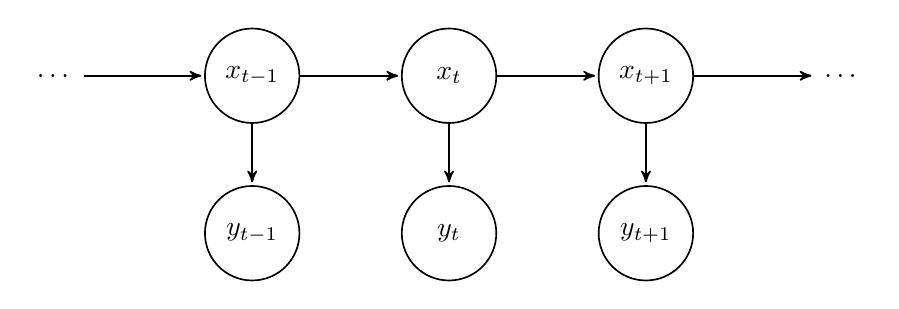
\begin{tikzpicture}[->,>=stealth',shorten >=1pt,auto,node distance=2.5cm,semithick]
    \node[state, minimum size=1.2cm]         (A)                    {$x_{t-1}$};
    \node[state, minimum size=1.2cm]         (B) [right of=A]       {$x_{t}$};
    \node[state, minimum size=1.2cm]         (C) [right of=B]       {$x_{t+1}$};

    \node[left of=A]  (prev) {$\dots$};
    \node[right of=C] (next) {$\dots$};

    \path (prev) edge node [above] {} (A)
    (A)    edge node [above] {} (B)
    (B)    edge node [above] {} (C)
    (C)    edge node [above] {} (next);

    \node [draw,circle,below of=A, node distance=2cm, minimum size=1.2cm] (WA) {$y_{t-1}$};
    \node [draw,circle,below of=B, node distance=2cm, minimum size=1.2cm] (WB) {$y_{t}$};
    \node [draw,circle,below of=C, node distance=2cm, minimum size=1.2cm] (WC) {$y_{t+1}$};

    \path (A) edge [->] (WA)
    (B) edge [->] (WB)
    (C) edge [->] (WC);
    \end{tikzpicture}
\end{center}
\caption{An HMM with 4 hidden states and 2 discrete emissions denoted by $x_1$ and $x_2$.}
\label{fig:HMM}
\end{figure}

We may also visualize conditional relationship with a graphical model in Figure \ref{fig:ergodic} representing a structure of HMM with 3 hidden states $\{S_1,S_2,S_3\}$ and 2 emission symbols $\{E_1,E_2\}$ where the nodes represent the relationship 
imposed by the transition matrix $\textbf{A}$ and emission matrix $\textbf{B}$:

\begin{figure}[htbp]
    \begin{center}
    \begin{tikzpicture}[]
    % states
    \node[state, minimum size=1.2cm] (s1) at (0,2) {$S_1$}
        edge [loop above]  node[auto,above] {$a_{11}$}();
    \node[state, minimum size=1.2cm] (s2) at (3,2) {$S_2$}
        edge [<-,bend right=45] node[auto,swap] {$a_{12}$} (s1)
        edge [->,bend left=45] node[auto,above] {$a_{21}$} (s1)
        edge [loop above] node[auto,above] {$a_{22}$} ();
    \node[state, minimum size=1.2cm] (s3) at (6,2) {$S_3$}
        edge [<-,bend right=70] node[auto,swap] {$a_{13}$} (s1)
        edge [->,bend left=60] node[auto,above] {$a_{31}$}(s1)
        edge [<-,bend right=45] node[auto,swap] {$a_{23}$} (s2)
        edge [->,bend left=45] node[auto,above] {$a_{32}$} (s2)
        edge [loop above] node[auto,above] {$a_{33}$} ();
    % observations
    \node[observation, minimum size=1cm] (y1) at (1.5,-1.5) {$E_1$}
        edge [lightedge] node[auto,below,xshift=-20pt] {$b_{S_1}(E_1)$} (s1)
        edge [lightedge] (s2)
        edge [lightedge] (s3);
    \node[observation, minimum size=1cm] (y2) at (4.5,-1.5) {$E_2$}
        edge [lightedge] (s1)
        edge [lightedge] (s2)
        edge [lightedge] node[auto,swap] {$b_{S_3}(E_2)$} (s3);
    \end{tikzpicture}
    \end{center}
    \caption{An HMM with 3 hidden states and 2 emission symbols denoted by $E_1$ and $E_2$.}
    \label{fig:ergodic}
    \end{figure}
    

There are 3 main assumptions of Hidden Markov Models as a consequence of the properties of Markov processes,
as suggested by \cite{Oliver2013} and \cite{}:

\begin{itemize}
    \item[1)] \textbf{Markov memoryless assumption} - this assumption states that the next hidden state $X_{t+1}$ depends only on the current state $X_t$, so that the transition probabilities are defined as:

        \begin{equation}
            \mathbb{P}(X_{t+1} = j| X_{t} = i,X_{t-1} = i_{t-1}, \ldots,X_{0} = i_0) = \mathbb{P}(X_{t+1} = j| X_{t} = i) \quad \forall i,j \in I
        \end{equation}

        It is also possible to assume that the states in HMM are dependent beyond the current state therefore giving rise to \textit{k-order HMM} 
        where the conditional distribution of the next state depends on the current state and the previous $k$ states $X_{t-k}, X_{t-k+1}, \ldots, X_{t-1}$. \cite{Capp2005}

    \item[2)] \textbf{Stationary assumption} - The transition matrix $\textbf{A}$ is time invariant s.t. transition probabilities only depend on the time interval between the transitions, 
    thus for all $t \neq s$:

        \begin{equation}
            \mathbb{P}(X_{t+1} = j| X_{t}= i) = \mathbb{P}(X_{s+1} = j| X_s = i) \quad \forall i,j \in I
        \end{equation}

        However, when we abstract from this assumption, we may consider a \textit{non-stationary HMM} where the transition matrix is time-dependent, i.e. depends on time index $t$.

    \item[3)] \textbf{Emission independence assumption} - Emissions are independent, s.t. if we have an emission sequence $\textbf{Y} = \{y_1,y_2,\ldots,y_T\}$ then:

        \begin{equation}
            \mathbb{P}(\textbf{Y}|X_1 = x_1,\ldots,X_T = x_T) = \prod_{t=1}^T \mathbb{P}(Y_t = y_t|X_t = x_t)
        \end{equation}

        When there is a dependence between the emissions in a way that the emission at time $t$ depends on the previous emissions, conditionally on the hidden state sequence $\{X_k\}$, $\{Y_k\}$
        forms a (non-homogeneous) Markov Chain, therefore jointly representing a generalization of HMM called \textit{Markov-switching Models}\footnote{Also, \textbf{Markov jump system}.}. \cite{Capp2005}

\end{itemize}

There are mainly 3 fundamental problems in HMM that need to be resolved as depicted by \cite{Oliver2013} and \cite{Ching2005}:
\begin{itemize}
\item[1.] \textbf{Evaluation problem} - Given a model denoted as $\theta = (\textbf{A},\textbf{B},\textbf{p})$ and an emission sequence $\textbf{Y} = y_1, y_2,\ldots,y_T$, how to efficiently compute the probability that the model generated the observation sequence, in other words, what is $\mathbb{P}(\textbf{Y}|\theta)$? 
\item[2.] \textbf{Decoding problem} - What is the most likely sequence of hidden states that could have generated the emission sequence \textbf{Y}? Thus, we would like to find $\textbf{X} = \underset{\textbf{X}}{\arg\max} \mathbb{P}(\textbf{Y},\textbf{X}|\theta)$, where $\textbf{X}$ is the hidden state sequence. 
\item[3.] \textbf{Learning problem} - Given a set of emission sequences find $\theta$ that best explains the emission sequence $\textbf{Y}$. Thus, find the vector of parameters $\theta$ that maximizes $\mathbb{P}(\textbf{Y}|\theta)$. 
\end{itemize}

The most traditional approaches in solving these 3 fundamental problems differ and one may not suffice in solving all three. 
The evaluation problem is usually solved by \textbf{Forward-Backward algorithm}\footnote{Focusing on the most widely used implementation called \textbf{alpha-beta algorithm}.}, the decoding problem by well-known \textbf{Viterbi algorithm} 
and the last learning problem by \textbf{Baum-Welsch algorithm} which is a special case of Expectation-maximization (EM) algorithm.
 All three algorithms are described in the following chapter.

\section{Gaussian HMM}

As shown in the last chapter the joint probability distribution of the complete 
data is not strictly concave and unimodal thus we can not guarantee the convergence to the global optimum.  
Fig 2.2 appropriately displays possible shape of the joint probability distribution of the complete data with multiple 
local optima of the log-likelihood function caused by the hidden states. 
Such probability distributions are often called mixture distributions. 

They were implicitly introduced in the last chapter while estimating the parameters of the Hidden Markov Model. 
Although, most of the time we consider unimodal distributions for our data it might not be the case for particular data sets.
Therefore, certain phenomena can be better described by mixture distributions, but their use should be justified theoretically or empirically. 
Statistical inferences about the subpopulations within the overall population require such tools in cases where the subpopulations significantly differ 
and may be interpreted the same way as hidden variables in case of Hidden Markov Models.
In this section, we first introduce the concept of \textit{mixture distributions}, then we will focus on \textit{Gaussian mixture models }
and their direct relation to \textit{Gaussian Hidden Markov Models}.

\subsection{Mixture Distributions}

Let $Y_j$ denote a p-dimensional random vector with probability density function $f(y_j)$ on $\mathbb{R}^p$  
selected from random sample $Y_1,\ldots,Y_n$. A realization of such a random vector is denoted by $y_j$.

Mixture distribution or density is defined as a convex combination of $g$ component distributions or densities respectively 
as follows:

\begin{equation}
f(y_j) = \sum_{i=1}^{g} \pi_i f_i(y_j)
\end{equation}

where $f_i(y_j)$ are component densities of the mixture and $\pi_i$ are mixing proportions or mixture weights with following properties:

\begin{equation}
    0 \leq \pi_i \leq 1 \quad \forall i \in \{1,2,\ldots,g\}
\end{equation}

and

\begin{equation}
    \sum_{i=1}^{g} \pi_i = 1
\end{equation}

Therefore, the density (3.1) of $f(y_j)$ is referred to as a g-component finite mixture density, conversely $F(y_j)$ 
as a g-component finite mixture distribution. 

Formula (3.1) assumes that the number of components $g$ is fixed. In many applications this is not the case, and we have to infer 
the number of components from the data. Furthermore, mixing proportions $\pi_i$ are also unknown and have to be estimated along with 
the respective parameters of the component densities $f_i(y_j)$.

Analogously to previous definition we can define a finite mixture of random variables $Y_j$ as follows:

\begin{equation}
    f(y_j,z) =  g(z) f(y_j|z)
\end{equation}

where $Z$ is defined as a random variable with multinomial distribution with a vector of parameters $\pi = \{\pi_1,\ldots,\pi_g\}$ and $g(z)$ as its probability density function.
Summing over all possible values of $Z$ we obtain the marginal density of random vector $Y_j$:

\begin{equation}
    f(y_j) = \sum_{i=1}^{g} P(Z=i) f(y_j|Z=i)
\end{equation}
    
where $P(Z=i) = \pi_i$ and $f(y_j|Z=i) = f_i(y_j)$ are the mixing proportions and component densities respectively Therefore
seeing the equivalence of Equation (3.1) and (3.4).

\subsection{Gaussian Mixture Models}
The Gaussian mixture model (GMM) is a probabilistic model that assumes all the data points are generated 
from a mixture of a finite number of Gaussian distributions. The component distributions are often chosen to be members of the same parametric family,
such as Gaussian distributions with respective mean and covariance parameter. Assuming that the number of components is $K$
the probability density function of the Gaussian mixture model can be expressed as follows:

\begin{equation}
    f(x|\mu,\Sigma) = \sum_{k=1}^{K} \pi_k \mathcal{N}(x|\mu_k, \Sigma_k)
\end{equation}

where $\mu_k$ and $\Sigma_k$ are the mean and covariance matrix (symmetric and positive semi-definite) of the $k$-th Gaussian component. 

Thus, the vector of parameters is $\theta = \{k \in \mathbb{N}: (\pi_k,\mu_k,\Sigma_k)\}$. Probability density function of each component of GMM depends on the dimensionality of the data.
Let the dimensionality of the data be $d>1$ then the random vector $Y=(y_1,\ldots,y_d)$ has the probability density function of the $k$-th component 
defined as following multivariate Gaussian distribution:

\begin{equation}
    f_k(y) = \frac{1}{{(2\pi)}^{d/2}|\Sigma_k|^{1/2}} \exp\left(-\frac{1}{2}{(y_j-\mu_k)}^T\Sigma_k^{-1}(y_j-\mu_k)\right)
\end{equation}

where $|\Sigma_k|$ denotes the determinant of the covariance matrix $\Sigma_k$.

\subsection{Motivating EM algorithm}
\cite{Bishop2006}
Given the data $\textbf{Y} = \{\textbf{Y}_1,\ldots,\textbf{Y}_N\}$, where each element is an independently and identically distributed 
p-dimensional random vector, s.t. $Y_n \in \mathbb{R}^p$ and:

\begin{equation}
    \textbf{Y}_n \sim \mathcal{N}_p(\mu, \Sigma) \quad \forall n \in \{1,\ldots,N\} 
\end{equation}

The goal is to estimate $\theta$ of the mixture model, 
i.e.\ for each mixture component $k$ we need to estimate its mean $\mu_k$, covariance matrix $\Sigma_k$ and mixing proportion $\pi_k$. 

Note that now we will assume that each element of random vector $\textbf{Y}_n$ is generated by one of the mixture components, and we know which one. 
This is called the complete data since we have information about the hidden variable $Z$ which indicates the component from which the data point was generated.
Therefore, the complete data likelihood function is defined as follows: 

\begin{equation} \label{eq:likelihood-gaussian}
    L_c(\theta|\textbf{Y},\textbf{Z}) = \prod_{i=1}^{N} \sum_{k=1}^{K} \pi_k \mathcal{N}(\textbf{Y}_i|\mu_k,\Sigma_k)
\end{equation}

and the log-likelihood function is:

\begin{equation}
    \ell_c(\theta|\textbf{Y},\textbf{Z}) = \sum_{n=1}^{N} \log \sum_{k=1}^{K} \pi_k \mathcal{N}(\textbf{Y}_n|\mu_k,\Sigma_k)
\end{equation}

Equation (3.10), shows that the log-likelihood function has a form of a sum of logarithms which results in no strict analytical solution for the maximum likelihood estimation of model parameters.

Given the assumption that we know the hidden variable $\textbf{Z}$ directly from the data defined as a K-dimensional random vector $\textbf{Z}=(z_1,\ldots,z_K)$ 
with multinomial distribution and parameters $\boldsymbol{\pi} = \{\pi_1,\ldots,\pi_K\}$, the log-likelihood function can be rewritten as follows:

\begin{equation}
    \ell_c(\theta|\textbf{Y},\textbf{Z}) = \sum_{i=1}^{N} \sum_{k=1}^{K} z_{ik} \left(\log \pi_k + \log \mathcal{N}(\textbf{Y}_n|\mu_k,\Sigma_k)\right)
\end{equation}

with variable $z_{ik}$ defined as follows:

\begin{equation}
    z_{ik} = \begin{cases}
        1 & \text{if } \textbf{Y}_i \text{ was generated by the } k\text{-th component} \\
        0 & \text{otherwise}
    \end{cases}
\end{equation}

also notice that for each sample, random vector $z_{i}$ is distributed identically and independently according to the multinomial distribution with vector of parameters $\boldsymbol{\pi}$.

\subsection{EM algorithm for GMM}

The EM algorithm for GMM is very similar to the one defined for Hidden Markov Models in the previous chapter. 
We start with the definition of the $\textbf{E-step}$ of the EM algorithm. The conditional expected complete 
data log-likelihood function given log-likelihood function by Equation (3.11) as follows:

\begin{equation}
    Q(\theta|\theta^{(t)}) = \mathbb{E}[\ell_c(\theta|\textbf{Y},\textbf{Z})|\textbf{Y},\theta^{(t)}]
\end{equation}

hence inserting Equation (3.11) into (3.13) we obtain:

\begin{equation}
    Q(\theta|\theta^{(t)}) = \sum_{i=1}^{N} \sum_{k=1}^{K} \mathbb{E}[z_{ik}|\textbf{Y}_i,\theta^{(t)}] \left(\log \pi_k + \log \mathcal{N}(\textbf{Y}_i|\mu_k,\Sigma_k)\right)
\end{equation}

where $\theta^{(t)}$ denotes the parameter vector at the $t$-th iteration of the algorithm and $\mathbb{E}[z_{ik}|\textbf{Y}_i,\theta^{(t)}]$ is the expected value of the hidden variable $z_{ik}$ given the data $\textbf{Y}_i$ and the parameter vector $\theta^{(t)}$.
The expected value of the hidden variable $z_{ik}$ is defined as follows:

\begin{equation} \label{eq:posterior_prob}
    \mathbb{E}[z_{ik}|\textbf{Y}_i,\theta^{(t)}] = P(z_{ik} = 1|Y_i,\theta^{(t)}) = \frac{\pi_k^{(t)} \mathcal{N}(\textbf{Y}_i|\mu_k^{(t)},\Sigma_k^{(t)})}{\sum_{j=1}^{K} \pi_j^{(t)} \mathcal{N}(\textbf{Y}_i|\mu_j^{(t)},\Sigma_j^{(t)})}
\end{equation}

where $\pi_k^{(t)}$, $\mu_k^{(t)}$ and $\Sigma_k^{(t)}$ are the mixing proportion, mean and covariance matrix of the $k$-th component at the $t$-th iteration of the algorithm respectively.
Taking a step back and looking at the Equation (3.5) we observe that the conditional expected value of $z_{ik}$ given data $\textbf{Y}_i$ 
and parameter vector $\theta^{(t)}$ is the posterior probability of the hidden variable $z_{ik}$.

The $\textbf{M-step}$ of the EM algorithm then aims to maximize the conditional expected complete data log-likelihood function $Q(\theta|\theta^{(t)})$ with respect to the parameter vector $\theta$.
Such maximization is formally defined as follows:

\begin{equation}
    \theta^{(t+1)} = \underset{\theta \in \Theta}{\arg\max} Q(\theta|\theta^{(t)})
\end{equation}

Taking partial derivatives of $Q(\theta|\theta^{(t)})$ with respect to the parameters $\pi_k$, $\mu_k$ and $\Sigma_k$ and setting them to zero we obtain the following equations:

\begin{equation}
    \hat{\pi}_k^{(t+1)} = \frac{1}{N} \sum_{i=1}^{N} \mathbb{E}[z_{ik}|\textbf{Y}_i,\theta^{(t)}]
\end{equation}

\begin{equation}
    \hat{\mu}_k^{(t+1)} = \frac{\sum_{i=1}^{N} \mathbb{E}[z_{ik}|\textbf{Y}_i,\theta^{(t)}] \textbf{Y}_i}{\sum_{i=1}^{N} \mathbb{E}[z_{ik}|\textbf{Y}_i,\theta^{(t)}]}
\end{equation}

\begin{equation}
    \hat{\Sigma}_k^{(t+1)} = \frac{\sum_{i=1}^{N} \mathbb{E}[z_{ik}|\textbf{Y}_i,\theta^{(t)}](\textbf{Y}_i - \mu_k^{(t+1)}){(\textbf{Y}_i - \mu_k^{(t+1)})}^T}{\sum_{i=1}^{N} \mathbb{E}[z_{ik}|\textbf{Y}_i,\theta^{(t)}]}
\end{equation}


\section{Poisson HMM}

\section{Context-sensitive HMM}
%!TEX root = ../thesis.tex
\chapter{Mixture Models}

\if
pdf
    \graphicspath{{Chapter3/Figs/Raster/}{Chapter3/Figs/PDF/}{Chapter3/Figs/}}
\else
    \graphicspath{{Chapter3/Figs/Vector/}{Chapter3/Figs/}}
\fi

As shown in the last chapter the joint probability distribution of the complete 
data is not strictly concave thus we can not guarantee the convergence to the global optimum. 
Approach we might take is to randomly initialize the parameters multiple times to see 
if the maxima of the log likelihood function increases. 
Fig 2.2 appropriately displays possible shape of the joint probability distribution of the complete data. 
There are visible multiple local optima of the log-likelihood function caused by the hidden states. 
Such probability distributions are often called mixture distributions. 

They were implicitly introduced in the last chapter while estimating the parameters of the Hidden Markov Model. 
Although, most of the time we consider unimodal distributions for our data since it may be justifiable empirically 
or considering the mixture distributions could unnecessarily complicate the computation 
for an indistinguishable improvement, the statistical inferences about the subpopulations 
within the population require such tools in cases where the subpopulations significantly differ.
However, in these models we pose no requirement of the knowledge about the number of subpopulations 
within the population or their actual distribution. They are interpreted the same way as for the HMM 
as hidden variables.

\section{Mixture Distributions}

Let $Y_j$ denote a p-dimensional random vector with probability density function $f(y_j)$ on $\mathbb{R}^p$  
selected from random sample $Y_1,\ldots,Y_n$. A realization of such a random vector is denoted by $y_j$.

Mixture distribution or density is defined as a convex combination of $g$ component distributions or densities respectively 
as follows:

\begin{equation}
f(y_j) = \sum_{i=1}^{g} \pi_i f_i(y_j)
\end{equation}

where $f_i(y_j)$ are component densities of the mixture and $\pi_i$ are mixing proportions or mixture weights with following properties:

\begin{equation}
    0 \leq \pi_i \leq 1 \quad \forall i \in \{1,2,\ldots,g\}
\end{equation}

and

\begin{equation}
    \sum_{i=1}^{g} \pi_i = 1
\end{equation}

Therefore, the density (3.1) of $f(y_j)$ is referred to as a g-component finite mixture density, conversely $F(y_j)$ 
as a g-component finite mixture distribution. 

Formula (3.1) assumes that the number of components $g$ is fixed. In many applications this is not the case, and we have to infer 
the number of components from the data. Furthermore, mixing proportions $\pi_i$ are also unknown and have to be estimated along with 
the respective parameters of the component densities $f_i(y_j)$.

Analogously to previous definition we can define a finite mixture of random variables $Y_j$ as follows:

\begin{equation}
    f(y_j,z) =  g(z) f(y_j|z)
\end{equation}

where $Z$ is defined as a random variable with multinomial distribution with a vector of parameters $\pi = \{\pi_1,\ldots,\pi_g\}$ and $g(z)$ as its probability density function.
Summing over all possible values of $Z$ we obtain the marginal density of random vector $Y_j$:

\begin{equation}
    f(y_j) = \sum_{i=1}^{g} P(Z=i) f(y_j|Z=i)
\end{equation}
    
where $P(Z=i) = \pi_i$ and $f(y_j|Z=i) = f_i(y_j)$ are the mixing proportions and component densities respectively Therefore
seeing the equivalence of Equation (3.1) and (3.4).

\section{Gaussian Mixture Models}
The Gaussian mixture model (GMM) is a probabilistic model that assumes all the data points are generated 
from a mixture of a finite number of Gaussian distributions. The component distributions are often chosen to be members of the same parametric family,
such as Gaussian distributions with respective mean and covariance parameter. Assuming that the number of components is $K$
the probability density function of the Gaussian mixture model can be expressed as follows:

\begin{equation}
    f(x|\mu,\Sigma) = \sum_{k=1}^{K} \pi_k \mathcal{N}(x|\mu_k, \Sigma_k)
\end{equation}

where $\mu_k$ and $\Sigma_k$ are the mean and covariance matrix (symmetric and positive semi-definite) of the $k$-th Gaussian component. 

Thus, the vector of parameters is $\theta = \{k \in \mathbb{N}: (\pi_k,\mu_k,\Sigma_k)\}$. Probability density function of each component of GMM depends on the dimensionality of the data.
Let the dimensionality of the data be $d>1$ then the random vector $Y=(y_1,\ldots,y_d)$ has the probability density function of the $k$-th component 
defined as following multivariate Gaussian distribution:

\begin{equation}
    f_k(y) = \frac{1}{{(2\pi)}^{d/2}|\Sigma_k|^{1/2}} \exp\left(-\frac{1}{2}{(y_j-\mu_k)}^T\Sigma_k^{-1}(y_j-\mu_k)\right)
\end{equation}

where $|\Sigma_k|$ denotes the determinant of the covariance matrix $\Sigma_k$.

\subsection{Motivating EM algorithm}

Given the data $\textbf{Y} = \{\textbf{Y}_1,\ldots,\textbf{Y}_N\}$, where each element is an independently and identically distributed 
p-dimensional random vector, s.t. $Y_n \in \mathbb{R}^p$ and:

\begin{equation}
    \textbf{Y}_n \sim \mathcal{N}_p(\mu, \Sigma) \quad \forall n \in \{1,\ldots,N\} 
\end{equation}

The goal is to estimate $\theta$ of the mixture model, 
i.e.\ for each mixture component $k$ we need to estimate its mean $\mu_k$, covariance matrix $\Sigma_k$ and mixing proportion $\pi_k$. 

Note that now we will assume that each element of random vector $\textbf{Y}_n$ is generated by one of the mixture components, and we know which one. 
This is called the complete data since we have information about the hidden variable $Z$ which indicates the component from which the data point was generated.
Therefore, the complete data likelihood function is defined as follows: 

\begin{equation} \label{eq:likelihood-gaussian}
    L_c(\theta|\textbf{Y},\textbf{Z}) = \prod_{i=1}^{N} \sum_{k=1}^{K} \pi_k \mathcal{N}(\textbf{Y}_i|\mu_k,\Sigma_k)
\end{equation}

and the log-likelihood function is:

\begin{equation}
    \ell_c(\theta|\textbf{Y},\textbf{Z}) = \sum_{n=1}^{N} \log \sum_{k=1}^{K} \pi_k \mathcal{N}(\textbf{Y}_n|\mu_k,\Sigma_k)
\end{equation}

Equation (3.10), shows that the log-likelihood function has a form of a sum of logarithms which results in no strict analytical solution for the maximum likelihood estimation of model parameters.

Given the assumption that we know the hidden variable $\textbf{Z}$ directly from the data defined as a K-dimensional random vector $\textbf{Z}=(z_1,\ldots,z_K)$ 
with multinomial distribution and parameters $\boldsymbol{\pi} = \{\pi_1,\ldots,\pi_K\}$, the log-likelihood function can be rewritten as follows:

\begin{equation}
    \ell_c(\theta|\textbf{Y},\textbf{Z}) = \sum_{i=1}^{N} \sum_{k=1}^{K} z_{ik} \left(\log \pi_k + \log \mathcal{N}(\textbf{Y}_n|\mu_k,\Sigma_k)\right)
\end{equation}

with variable $z_{ik}$ defined as follows:

\begin{equation}
    z_{ik} = \begin{cases}
        1 & \text{if } \textbf{Y}_i \text{ was generated by the } k\text{-th component} \\
        0 & \text{otherwise}
    \end{cases}
\end{equation}

also notice that for each sample, random vector $z_{i}$ is distributed identically and independently according to the multinomial distribution with vector of parameters $\boldsymbol{\pi}$.

\subsection{EM algorithm for GMM}

The EM algorithm for GMM is very similar to the one defined for Hidden Markov Models in the previous chapter. 
We start with the definition of the $\textbf{E-step}$ of the EM algorithm. The conditional expected complete 
data log-likelihood function given log-likelihood function by Equation (3.11) as follows:

\begin{equation}
    Q(\theta|\theta^{(t)}) = \mathbb{E}[\ell_c(\theta|\textbf{Y},\textbf{Z})|\textbf{Y},\theta^{(t)}]
\end{equation}

hence inserting Equation (3.11) into (3.13) we obtain:

\begin{equation}
    Q(\theta|\theta^{(t)}) = \sum_{i=1}^{N} \sum_{k=1}^{K} \mathbb{E}[z_{ik}|\textbf{Y}_i,\theta^{(t)}] \left(\log \pi_k + \log \mathcal{N}(\textbf{Y}_i|\mu_k,\Sigma_k)\right)
\end{equation}

where $\theta^{(t)}$ denotes the parameter vector at the $t$-th iteration of the algorithm and $\mathbb{E}[z_{ik}|\textbf{Y}_i,\theta^{(t)}]$ is the expected value of the hidden variable $z_{ik}$ given the data $\textbf{Y}_i$ and the parameter vector $\theta^{(t)}$.
The expected value of the hidden variable $z_{ik}$ is defined as follows:

\begin{equation} \label{eq:posterior_prob}
    \mathbb{E}[z_{ik}|\textbf{Y}_i,\theta^{(t)}] = P(z_{ik} = 1|Y_i,\theta^{(t)}) = \frac{\pi_k^{(t)} \mathcal{N}(\textbf{Y}_i|\mu_k^{(t)},\Sigma_k^{(t)})}{\sum_{j=1}^{K} \pi_j^{(t)} \mathcal{N}(\textbf{Y}_i|\mu_j^{(t)},\Sigma_j^{(t)})}
\end{equation}

where $\pi_k^{(t)}$, $\mu_k^{(t)}$ and $\Sigma_k^{(t)}$ are the mixing proportion, mean and covariance matrix of the $k$-th component at the $t$-th iteration of the algorithm respectively.
Taking a step back and looking at the Equation (3.5) we observe that the conditional expected value of $z_{ik}$ given data $\textbf{Y}_i$ 
and parameter vector $\theta^{(t)}$ is the posterior probability of the hidden variable $z_{ik}$.

The $\textbf{M-step}$ of the EM algorithm then aims to maximize the conditional expected complete data log-likelihood function $Q(\theta|\theta^{(t)})$ with respect to the parameter vector $\theta$.
Such maximization is formally defined as follows:

\begin{equation}
    \theta^{(t+1)} = \underset{\theta \in \Theta}{\arg\max} Q(\theta|\theta^{(t)})
\end{equation}

Taking partial derivatives of $Q(\theta|\theta^{(t)})$ with respect to the parameters $\pi_k$, $\mu_k$ and $\Sigma_k$ and setting them to zero we obtain the following equations:

\begin{equation}
    \hat{\pi}_k^{(t+1)} = \frac{1}{N} \sum_{i=1}^{N} \mathbb{E}[z_{ik}|\textbf{Y}_i,\theta^{(t)}]
\end{equation}

\begin{equation}
    \hat{\mu}_k^{(t+1)} = \frac{\sum_{i=1}^{N} \mathbb{E}[z_{ik}|\textbf{Y}_i,\theta^{(t)}] \textbf{Y}_i}{\sum_{i=1}^{N} \mathbb{E}[z_{ik}|\textbf{Y}_i,\theta^{(t)}]}
\end{equation}

\begin{equation}
    \hat{\Sigma}_k^{(t+1)} = \frac{\sum_{i=1}^{N} \mathbb{E}[z_{ik}|\textbf{Y}_i,\theta^{(t)}](\textbf{Y}_i - \mu_k^{(t+1)}){(\textbf{Y}_i - \mu_k^{(t+1)})}^T}{\sum_{i=1}^{N} \mathbb{E}[z_{ik}|\textbf{Y}_i,\theta^{(t)}]}
\end{equation}

\subsection{Markov Chain Monte Carlo}

Although, EM algorithm is a very powerful tool for estimating parameters of the mixture model,
it is not guaranteed to converge to the global optimum of the log-likelihood function. Therefore, 
we will introduce a Markov Chain Monte Carlo (MCMC) method for estimating the parameters of the mixture model by 
sampling from the posterior distribution of the parameters. As opposed to the previous subsection, the MCMC method 
also provides a measure of uncertainty of the estimated parameters.     

\subsubsection{Metropolis-Hastings Algorithm}

The Metropolis-Hastings algorithm is a Markov Chain Monte Carlo method for sampling from a probability distribution. 
The algorithm is based on the idea of constructing a Markov chain that has a stationary distribution equal to the target distribution.
The algorithm is defined as follows:

\begin{enumerate}
    \item Initialize the Markov chain with an arbitrary state $\theta^{(0)}$.
    \item For $t = 1,2,\dots$:
    \begin{enumerate}
        \item Sample a candidate state $\theta^*$ from a proposal distribution $q(\theta^*|\theta^{(t-1)})$.
        \item Compute the acceptance probability $\alpha(\theta^{(t-1)},\theta^*)$.
        \item Sample a random number $u$ from the uniform distribution $U(0,1)$.
        \item If $u < \alpha(\theta^{(t-1)},\theta^*)$ then set $\theta^{(t)} = \theta^*$, otherwise set $\theta^{(t)} = \theta^{(t-1)}$.
    \end{enumerate}
\end{enumerate}

The last step (d) is often called {\it Metropolis rejection} and the acceptance probability $\alpha(\theta^{(t-1)},\theta^*)$ in step (b) is defined as follows:

\begin{equation} \label{eq:hastings_ratio}
    \alpha(\theta^{(t-1)},\theta^*) = \min \left(1,\frac{p(\theta^*)q(\theta^{(t-1)}|\theta^*)}{p(\theta^{(t-1)})q(\theta^*|\theta^{(t-1)})}\right)
\end{equation}

where $p(\theta)$ is the target distribution and $q(\theta^*|\theta^{(t-1)})$ is the proposal distribution from which we can easily sample.
The second term in the minimum function of Equation \ref{eq:hastings_ratio} is called Hastings ratio. Metropolis rejection ensures here that 
the probability of accepting a candidate state $\theta^*$ is equal to $\alpha(\theta^{(t-1)},\theta^*)$ and rejecting it with probability $1 - \alpha(\theta^{(t-1)},\theta^*)$.
Proposal distributions are usually chosen to be symmetric, i.e. $q(\theta^*|\theta^{(t-1)}) = q(\theta^{(t-1)}|\theta^*)$, 
so that the computation of Hastings ratio is simplified (to Metropolis ratio) and the acceptance probability is therefore following:

\begin{equation}
    \alpha(\theta^{(t-1)},\theta^*) = \min \left(1,\frac{p(\theta^*)}{p(\theta^{(t-1)})}\right)
\end{equation}

Given the Gaussian mixture model, we can use the Metropolis-Hastings algorithm to sample from the posterior distribution of the parameters $\pi_k$, $\mu_k$ and $\Sigma_k$. 
The target distribution is the posterior distribution of the parameters, i.e. $p(\pi_k,\mu_k,\Sigma_k|\textbf{Y})$.
This distribution is proportional to the product of the prior distribution and the likelihood function, i.e. $p(\pi_k,\mu_k,\Sigma_k|\textbf{Y}) \propto p(\pi_k,\mu_k,\Sigma_k)p(\textbf{Y}|\pi_k,\mu_k,\Sigma_k)$ as follows from the Bayes' theorem.
The prior distribution is the conjugate prior of the multivariate Gaussian distribution, i.e. the Normal-Wishart distribution when we want to infer both the mean and the covariance matrix of the Gaussian distribution.
The Normal-Wishart distribution is defined as follows:

\begin{equation}
    \mathcal{NW}(\mu,\Sigma|\mu_0,\kappa_0,\nu_0,\Lambda_0) = \mathcal{N}(\mu|\mu_0,(\kappa_0\Sigma)^{-1})\mathcal{W}(\Sigma|\nu_0,\Lambda_0)
\end{equation}

where $\mu_0$ is the prior mean, $\kappa_0$ is the prior precision, $\nu_0$ is the prior degrees of freedom and $\Lambda_0$ is the prior scale matrix.
The likelihood function is the product of the component Gaussian distributions given by Equation \ref{eq:likelihood-gaussian}. Together with the prior distribution, the posterior distribution is given by the following:

\begin{equation}
    p(\pi_k,\mu_k,\Sigma_k|\textbf{Y}) \propto \prod_{i=1}^{N} \prod_{k=1}^{K} \left[ \pi_k \mathcal{N}(\textbf{Y}_i|\mu_k,\Sigma_k) \right]^{\mathbb{E}[z_{ik}|\textbf{Y}_i,\theta^{(t)}]} \mathcal{NW}(\mu_k,\Sigma_k|\mu_0,\kappa_0,\nu_0,\Lambda_0)
\end{equation}

where $\mathbb{E}[z_{ik}|\textbf{Y}_i,\theta^{(t)}]$ is the posterior probability of the $i$-th observation belonging to the $k$-th component Gaussian distribution given the current estimate of the parameters $\theta^{(t)}$ as per Equation \ref{eq:posterior_prob}.
The proposal distribution is often defined as a multivariate Gaussian distribution with mean $\theta^{(t-1)}$ and covariance matrix $\Sigma$ which effects the convergence of the algorithm since it determines the size of the step taken in the parameter space. 
If $\Sigma$ is too small the algorithm might not explore the parameter space sufficiently and the Markov chain might get stuck in a local optimum. On the other hand, if $\Sigma$ is too large then the Markov chain might not converge at all. 
The choice of the proposal distribution is not unique, and it is usually determined empirically given some knowledge about the target distribution. 
Initialization of the Markov chain in the first step of the algorithm is also crucial since if the initial state is far from the region of high probability of the target distribution then the Markov chain might not converge at all.
Lastly, notice that the samples from proposal conditional distribution are correlated since the next state of the Markov chain depends on the previous state which is a consequence of the Markov property and differs from the independent sampling of the parameters.

In summary, the Metropolis-Hastings algorithm is very flexible and simple to implement, and it is often used as a baseline for more sophisticated MCMC methods. 
There are several variants of the Metropolis-Hastings algorithm, e.g. Metropolis-within-Gibbs sampling, which is a special case of the Metropolis-Hastings algorithm where the proposal distribution is chosen to be the conditional distribution of the parameters given the current state of the Markov chain.


\subsubsection{Gibbs Sampling}


%%!TEX root = ../thesis.tex
\chapter{Trading strategies based on Hidden Markov Models}

\if
pdf
    \graphicspath{{Chapter5/Figs/Raster/}{Chapter5/Figs/PDF/}{Chapter5/Figs/}}
\else
    \graphicspath{{Chapter5/Figs/Vector/}{Chapter5/Figs/}}
\fi

\section{Selected Market Emissions}

	There is a huge number of observable variables that one could abstract from cryptocurrency market. A possibility of discrete states within the given state space is plausible and feasible, it would, given our model constraints, provide poor inference since additional information would remain hidden. Imagine a situation where our observable states are defined as a relative change in price or a sudden drop/uprise in the traded volume on the exchange. In order to discreticize our states and construct transition and emission probabilities we are forced to construct intervals that would well represent the boundaries upon which the model defines structure and predictions. 
	
Assuming that the price increase in   the idea predefined Hidden Markov Model will assume
	
	However it is much more efficient to assume continuity in our predefined observable states. It is nowadays empirically proved, as in (citace) that using technical indicators as predictors for the future spot price yields more accurate machine learning models. As will be demonstrated each of the technical indicators can be classified into several families of indicators, such as momentum, volume, volatility and cycle indicators. For our purposes we will consider mainly momentum indicators that are calculated using Open, High, Low, Close prices (hereinafter "OHLC") and Volume indicators. There is a huge variety of technical indicators to choose from therefore the selection was made according the most used and well known indicators or their transformed versions. 

In our case we will consider following observable states that will be defined and elaborated on in the upcoming sections:

\begin{itemize}
\item[1)] Moving Average Convergence/Divergence (MACD)
\item[2)] Stochastic Oscillator
\item[3)] Chaikin Oscillator 
\item[4)] Relative Strength Index (RSI)
\item[5)] Aroon Oscillator 
\end{itemize}


\subsection{Moving Average Convergence Divergence}

Also knows as MACD is a trend-following momentum indicator that represents the differences between two exponential moving averages (hereinafter "EMA"). The most common and traditional moving averages are 26-period EMA and 12-period EMA. 

The indicator is often used with so-called ""signal line" that is constructed as a 9-period EMA and is used as a trigger for a buy and sell signal. In practical application a trader decides to buy a stock if the signal line crosses MACD line from above and sell if it crosses from below, assuming simplistic trading strategy using only MACD. EMA also called exponentially weighted moving average is a type of moving average that differs from weighted moving average WMA by the distribution of weights to past observations. While WMA considers the linearly decreasing distribution of weights, the EMA assumes exponential decrease in weights. Furthermore it is necessary to elaborate over the values of weights because it might not always be unambiguous. WMA distributes weights chronologically and linearly, e.g. 10-period WMA gives weight 1 to the earliest observation and 10 to the most recent observation, the case within EMA is often not that simple. The weights given to each observation are computed as $(1 - \lambda)^i$ where $i \in \mathbb{N}_0$ and is bounded from above by the assumed period of interest, e.g. 3, 10, 26-period denoted as T for the sake of . As $i$ increases identically with the time lag the value of weights decreases. The important role that ought to be questioned is the parameter $\lambda$ that is defined as $\frac{k}{T+1}$ where k represents the so called "smoothing" parameter. Traders and analysts use value 2 for the smoothing parameter but the number may be defined on the interval $(0,T)$. Higher values of k mean bigger weights given to most recent observations. 

The Figure 2.1 illustrates MACD line, signal line as well as "MACD histogram" which is displayed as a bar chart indicating the difference of the former ones. Traders use such a distance to identify whether the bullish or bearish momentum is high, i.e. bigger the distances of these two lines higher the price momentum.

MACD has its unfortunate limitations that mainly arise from the non-trending moments. When the price enters sideways movement the MACD histogram signals decreases distances between MACD and signal line, the trend reversal is possible but the price moves sideways which eventually results in false positive signal. Moreover when the price moves sideways for longer periods MACD may signal too many false trend reversals. The most common practice for traders is to combine MACD signals with other indicators such as Relative Strength index (RSI) that measures overbought or oversold market. The RSI uses average price gains and losses usually over 14 periods and yields values between 0 and 100, indicating overbought market for values 70 (80) to 100 and 30 (20) to 0 for oversold market. The idea is that when the distances between MACD line and signal line increase and RSI signals overbought market the trader might consider this as a strong trend reversal signal. The idea is that signals from MACD strategy often produce false signals when price suddenly moves sideways and RSI helps to indicate the false positive signal. 

\begin{figure}[ht]

\begin{center}
	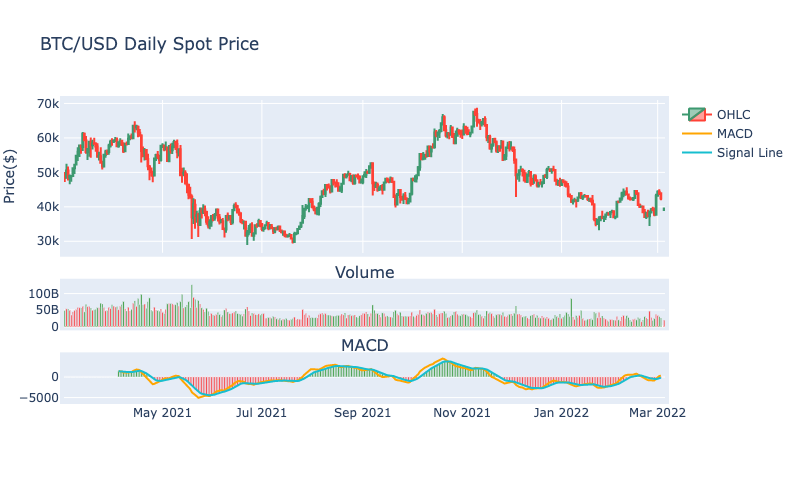
\includegraphics[width=0.9\textwidth]{Figs/MACD.png}
\end{center}

\caption{\textit{ Candlestick graph of daily spot price of BTC/USD from March 2021 to March 2022 with subplot containing two lines for MACD and Signal line and a bar chart as their difference}}

\end{figure}

\subsection{Stochastic Oscillator}

	A Stochastic Oscillator is a momentum indicator that compares the most recent closing price of a security with its predeceasing ones. Naturally, the range of preceding closing prices or the range of closing prices is 14 periods but it is regular that such an assumption is often edited to best fit the current needs of a trader. Also slight variation in taking the (weighted) moving average of the oscillator values is often introduced. The indicator is used to generate trading signals that refer to the current overbought state of the market, which means that the indictor values range from 0 to 100 where the values closer to the number 0 indicate oversold market and inversely values closer to 100 overbought market. 
	
Stochastic Oscillator is computed as follows:

\begin{equation}
SO_{t} = \frac{C_{t-1} - L_{14}}{H_{14} - L_{14}}
\end{equation}

where $C_{t-1}$ denotes the most recent closing price of a security, $H_{14}$ and $L_{14}$ are the highest and lowest price traded during 14-period interval respectively. $SO_{t}$ is sometimes referred to as a "fast" stochastic indicator. As said before this interval may be changed arbitrarily. Traders also developed so called "slow" Stochastic Oscillator which is defined as a 3-period moving average of $SO_{t}$. Thus when Stochastic Oscillator crosses the smooth "Slow" Stochastic Oscillator a trading signal is generated.

Considering values above 80, the indicator signals overbought market and oversold market when the value drops below 20. Although it remains to hold true that the indicator often produces false indications that may be caused by periods of time where the price remains overbought/oversold for some time and trading with respect to such oscillator may result in losses. It is rather recommended to observe the values of stochastic oscillator and use it for trend reversal indication. 

\begin{figure}[ht]

\begin{center}
	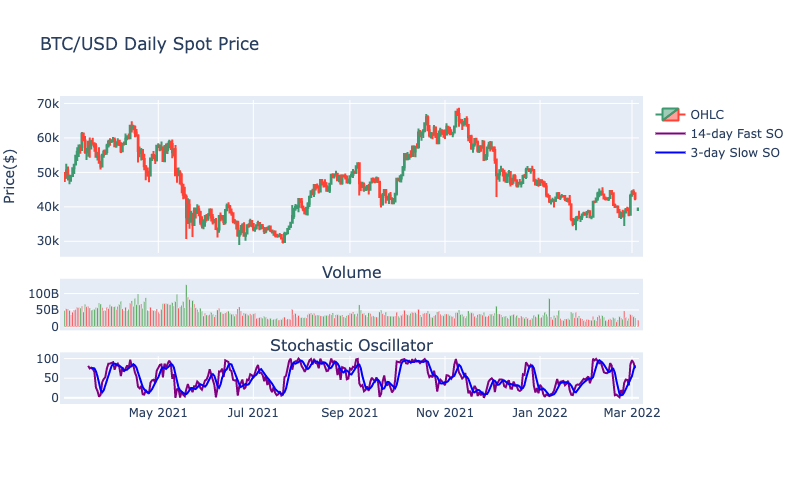
\includegraphics[width=0.9\textwidth]{Figs/Stochastic.png}
\end{center}

\caption{\textit{ Candlestick graph of daily spot price of BTC/USD from March 2021 to March 2022 with subplot with line indicating Stochastic Oscillator}}

\end{figure}

\newpage

\subsection{Chaikin Oscillator}

Chaikin Oscillator is a momentum based indicator of the Accumulation/Distribution Line (hereinafter "A/D line"), which is a cumulative indicator that aims to identify potential divergences between stock price and trading volume. The oscillator is calculated as a difference between 3- day and 10-day Exponential Moving Average of A/D line. 

\vspace{0.5cm}

The calculation of the Chaikin Oscillator may be broken down into several steps:
\begin{itemize}
\item[(i)] First, we ought to calculate the Money Flow Multiplier for each time step denoted by "N".

\begin{equation}
N_{t} = \frac{(Close_{t} - Low_{t}) - (High_{t} - Close_{t})}{High_{t} - Low_{t}}
\end{equation}

\item[(ii)] Now we may multiply $N_t$ by the trading volume in given period of time to get the Money Flow Volume denoted as $M_t$. With that we recursively construct the A/D line as:

\begin{equation}
ADL_t = M_{t-1} + M_t
\end{equation}

\item[(iii)] Given the constructed A/D line, we compute the Chaikin Oscillator values as a difference of 3-day and 10-day exponential moving averages.

\begin{equation}
CO_t = \frac{\sum_{i=0}^{3} {(1-\alpha)}^i*Close_{t-i}}{\sum_{i=0}^{3} {(1-\alpha)}^i} - \frac{\sum_{i=0}^{10} {(1-\beta)}^i*Close_{t-i}}{\sum_{i=0}^{10} {(1-\beta)}^i}
\end{equation}

where we assume that the weights denoted as $\alpha$ and $\beta$ are computed as $2/(days + 1)$. Numerator as a smoothing factor is often declared as 2. However, the indicator may be set to absolutely different number between 0 and 1 according to the needs and assumptions made by the trader/analyst, therefore setting the parameter close to 1 is putting more weight to the most recent price.

One way to interpret the indicator is to trade with respect to the time when the Chaikin Oscillator crosses zero from below and above which signals buy and sell signals respectively.

\end{itemize}


\begin{figure}[ht]

\begin{center}
	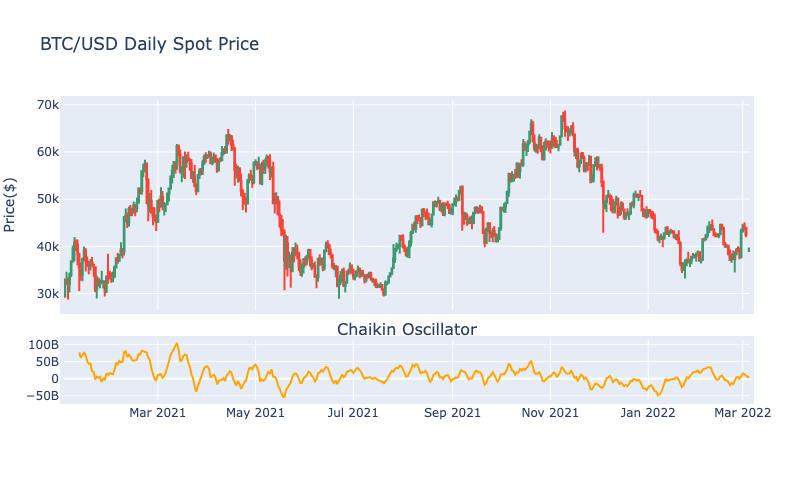
\includegraphics[width=0.9\textwidth]{Figs/Chaikin.png}
\end{center}

\caption{\textit{ Candlestick graph of daily spot price of BTC/USD from March 2021 to March 2022 with subplot indicating Chaikin Oscillator}}

\end{figure}


\subsection{Relative Strength Index}

Given the recent price changes Relative Strength Index measures its magnitude in order to indicate the overbought or oversold market. In technical analysis such indicator is represented by an oscillator ranging from values 0 to 100. Empirically 
it was determined that values above 70 and below 30 signal overbought and oversold asset respectively. Therefore, we may also use RSI to produce buy and sell signals from former logic, which means that when the RSI crosses 30 from below, buy signal is generated as well as sell signal in case it crosses 70 from above. We also could measure the strength and continuation of the trend for cases in which the RSI crosses value of 50. Such interpretation results from the RSI formula where the value of 50 means that the average gain equals the average loss in the last period.

The formula below explains the procedure within which the values of RSI are calculated. It is obvious that the RSI rises as the number of positive closing prices increases, i.e. the relative change in prices is positive, and falls if otherwise. The standard time interval for  the calculation is 14 preceding periods with respect to $t$, hereby denoted as $T$.

\begin{equation}
RSI_t = 100- \frac{100}{1+r_t} 
\end{equation}
 
 where r is a ratio of average gains and losses as follows:
 
\begin{equation}
 r_t = \abs{\frac{\sum_{i=1}^{T}(\frac{P_{t-i+1}}{P_{t-i}}-1)\mathbbm{1}_{[P_{t-i+1} - P_{t-i} > 0]}}{\sum_{i=1}^{T}(\frac{P_{t-i+1}}{P_{t-i}}-1) \mathbbm{1}_{[P_{t-i+1} - P_{t-i} < 0]}}}
\end{equation}

given that $P_t$ denotes the value of an asset at time $t$.

As stated before there are several drawbacks of using the RSI as a trading indicators only by itself, it happens that the price usually rises and stays overbought for a substantial period of time in times of significant and strong bullish trend. RSI as an oscillator is used as an auxiliary trading tool below the price chart:

\begin{figure}[ht]

\begin{center}
	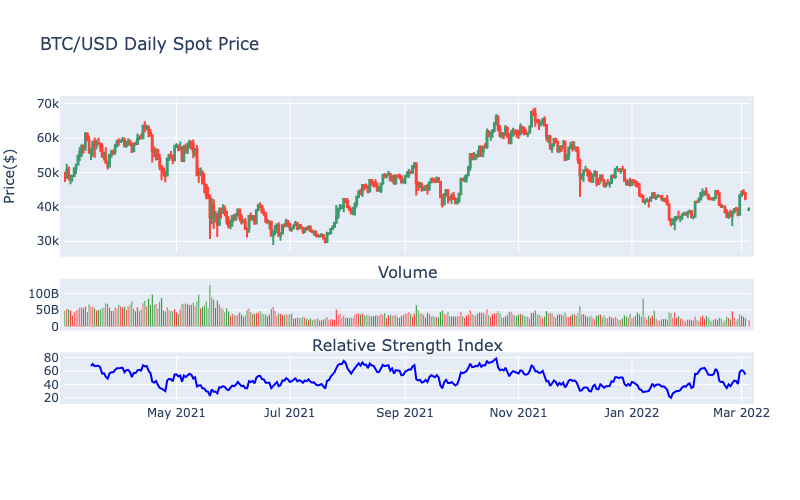
\includegraphics[width=0.9\textwidth]{Figs/RSI.png}
\end{center}

\caption{\textit{ Candlestick graph of daily spot price of BTC/USD from March 2021 to March 2022 with a subplot containing  RSI}}

\end{figure}

\subsection{Aroon Indicator}

Aroon indicator is used for trend reversal identification and a measure of its strength. Indicator is composed out of two lines aroon up and aroon down that measure the time between new highs or lows respectively. Alternatively, they measure the strength of a bullish or bearish trend. Obviously the main idea of the indicator is based upon the fact that bullish trends are naturelly formed by subsequently creating new highs while bearish trends form new lows. Aroon Up and Aroon Down are computed as follows:

\begin{equation}
Aroon Up = \frac{25 - h}{25} * 100
\end{equation}
 
\begin{equation}
Aroon Down = \frac{25 - l}{25} * 100
\end{equation}

Where $h$ represents the number of periods from the last 25-period High and $l$ the number of periods from last 25-period Low. 

The interpretation of the indicator is very intuitive since the situation in which the Aroon Up line is above Aroon Down line signals bullish trend and when these two lines cross the signal of the trend reversal is generated. That also implies that for higher values of Aroon Up the bigger the strength and for lower values the uptrend is weaker and vice versa. In practice the crossover of these two lines is what generates the buy or sell signals, i.e.\ if Aroon Up crosses Aroon Down line from below a buy signal is generated and vice versa. 

Although, Figure 2.4 graphically illustrates the Aroon Up and Down lines well, it is simpler to transform these two lines into one oscillator that would produce buy or sell signal in the case of zero crossover from above and from below. That is achieved by subtracting Aroon Up and Aroon Down line creating Aroon Oscillator.

\begin{figure}[ht]
\begin{center}
	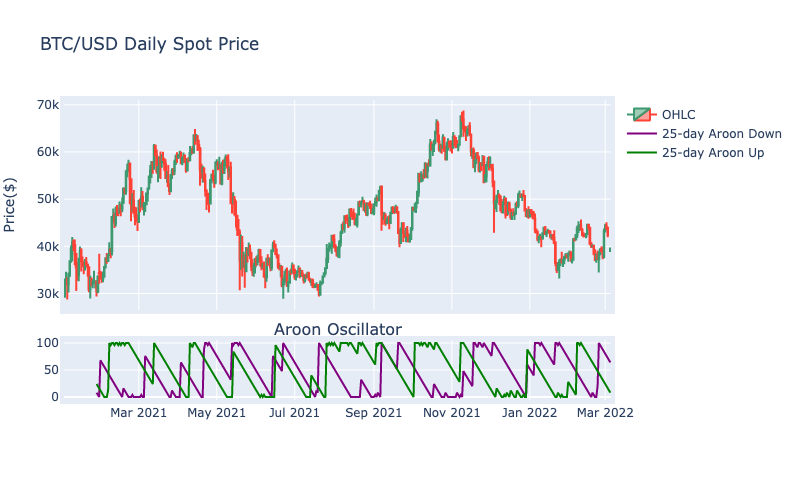
\includegraphics[width=0.9\textwidth]{Figs/Aroon.png}
\end{center}
\caption{\textit{Candlestick graph of daily spot price of BTC/USD from March 2021 to March 2022 with subplots containing two lines for Aroon Up/Down Indicator and Aroon Oscillator}}
\end{figure}

\section{Market regimes and trading strategies}

\subsection{Market states}

\subsection{Trading strategies}
%%!TEX root = ../thesis.tex
\chapter{Trading strategies based on Hidden Markov Models}

\if
pdf
    \graphicspath{{Chapter5/Figs/Raster/}{Chapter5/Figs/PDF/}{Chapter5/Figs/}}
\else
    \graphicspath{{Chapter5/Figs/Vector/}{Chapter5/Figs/}}
\fi


\section{Market regimes and trading strategies}

\subsection{Market states}

\subsection{Trading strategies}

%\include{Chapter6/chapter6}
%\include{Chapter7/chapter7}



% ********************************** Back Matter *******************************
% Backmatter should be commented out, if you are using appendices after References
%\backmatter

% ********************************** Bibliography ******************************
\begin{spacing}{0.9}

% To use the conventional natbib style referencing
% Bibliography style previews: http://nodonn.tipido.net/bibstyle.php
% Reference styles: http://sites.stat.psu.edu/~surajit/present/bib.htm

\bibliographystyle{apalike}
%\bibliographystyle{unsrt} % Use for unsorted references  
%\bibliographystyle{plainnat} % use this to have URLs listed in References
\cleardoublepage
\bibliography{References/references} % Path to your References.bib file


% If you would like to use BibLaTeX for your references, pass `custombib' as
% an option in the document class. The location of 'reference.bib' should be
% specified in the preamble.tex file in the custombib section.
% Comment out the lines related to natbib above and uncomment the following line.

%\printbibliography[heading=bibintoc, title={References}]


\end{spacing}

% ********************************** Appendices ********************************

\begin{appendices} % Using appendices environment for more functunality

%!TEX root = ../thesis.tex
% ******************************* Thesis Appendix A ****************************

\chapter{Maximum likelihood results}
%!TEX root = ../thesis.tex
% ******************************* Thesis Appendix B ********************************

\chapter{Python code}





\end{appendices}

% *************************************** Index ********************************
\printthesisindex % If index is present

\end{document}
